\comm{
	\section{Lax Pairs and Double Bracket Flows}
\subsection{Definition of a Lax Pair}
Two operator \(A\) and \(B\) are said to form a lax pair if they satisfy the equation
\begin{equation}\begin{aligned}
	\label{lax}
	\frac{\mathrm{d}A(t)}{\mathrm{d}t} = \left[B(t), A(t)\right]
\end{aligned}\end{equation}
\subsection{Unitary Nature of the Flow}
It can be shown that this defines a unitary time evolution on \(A(t)\), in the following manner. Let \(U(t,t_0)\) be the unitary operator that carries this evolution through. We then need to construct a \(U(t,t_0)\). 
\begin{equation}
	A(t) = U(t,t_0) A(t_0) U^\dagger (t,t_0)
\end{equation}
where \(A(t_0)\) is the operator \(A\) at a particular time \(t_0\). The time change of \(A\) can then be written as
\begin{equation}\begin{aligned}
	\frac{\mathrm{d}A(t)}{\mathrm{d}t} &= \frac{\mathrm{d}U(t, t_0)}{\mathrm{d}t} A(t_0) U^\dagger(t,t_0) + U(t,t_0) A(t_0) \frac{\mathrm{d}U^\dagger(t, t_0)}{\mathrm{d}t}\\
					   &= \frac{\mathrm{d}U(t, t_0)}{\mathrm{d}t} U^\dagger(t,t_0) A(t) + A(t) U(t,t_0) \frac{\mathrm{d}U^\dagger(t, t_0)}{\mathrm{d}t} && \left[ A(t) = U A U^\dagger\right]\\ 
					   &= \frac{\mathrm{d}U(t, t_0)}{\mathrm{d}t} U^\dagger(t,t_0) A(t) - A(t) \frac{\mathrm{d}U(t, t_0)}{\mathrm{d}t} U^\dagger(t,t_0) && \left[ U U^\dagger = 1 \right]\\ 
					   &= \left[\frac{\mathrm{d}U(t, t_0)}{\mathrm{d}t} U^\dagger(t,t_0), A(t)\right]
\end{aligned}\end{equation}
Looking at the definition of a lax pair, we can now make the connection
\begin{equation}\begin{aligned}
	\label{unitary}
	B(t) = \frac{\mathrm{d}U(t, t_0)}{\mathrm{d}t} U^\dagger(t,t_0)
\end{aligned}\end{equation}

\textbf{The equation of motion characterised by the lax pair eq.~\ref{lax} can thus be said to generate a family of unitarily connected operators \(A(t)\), related by the unitaries defined by eq.~\ref{unitary}. A direct corrolary is that the spectrum of \(A(t)\) is preserved during this evolution.}
\subsection{Double Bracket Flow}
The double bracket flows correspond to a special choice of the operator \(B(t)\): \(B(t) \equiv \left[A(t), C\right]\). A consequence of this choice is that the lax pair evolution then serves to minimize the commutator \(\left[A(t), C\right]\). To see how, we first write down a function
\begin{equation}
	\label{minfunc}
	\chi \equiv \text{Tr}\left(\left[A(t) - C\right]^2\right) = \text{Tr}\left[A(t)^2 + C^2 - A(t) C - C A(t)\right]
\end{equation}
Since \(A^2(t) = U A^2 U^\dagger\), we get \(\text{Tr}(A^2(t)) = \text{Tr}(A)\). Also, from the cyclic nature of trace, we can write \(\text{Tr}(A(t)C)=\text{Tr}(CA(t))\). These considerations (and the fact that \(C\) does not depend on \(t\)) allows us to write
\begin{equation}
	\frac{\mathrm{d} \chi}{\mathrm{d}t} = -2\text{Tr}\left(\frac{\mathrm{d} A(t)}{\mathrm{d}t}\;C\right) = -2\text{Tr}\left(\left[B(t),A(t)\right] C\right)
\end{equation}
Using the cyclic property of trace, this becomes
\begin{equation}\begin{aligned}
	\text{Tr}\left(\left[B(t),A(t)\right] C\right) &= \text{Tr}\left(B(t)A(t) C - A(t) B(t)C\right)\\
						       &= \text{Tr}\left(B(t)A(t) C - B(t)A(t) C\right)\\
						       &= \text{Tr}\left(B(t)\left[A(t), C\right]\right)\\
\end{aligned}\end{equation}
If we now substitute the choice of \(B(t)\) we made above, we get
\begin{equation}
	\frac{\mathrm{d} \chi}{\mathrm{d}t} = -2\text{Tr}\left(\left[A(t), C\right]^2\right) = -2\text{Tr}\left(B(t)^2\right) \leq 0
\end{equation}
Since \(\chi\), the way it is defined, must necessarily be positive semi-definite for all \(t\), it has a global minimum at \(\chi = 0\). Since the derivative \(\frac{\mathrm{d} \chi}{\mathrm{d}t}\) is always negative, it will take \(\chi\) towards its minimum. At the minimum, the time derivative must vanish, otherwise \(\chi(t)\) will become negative. This gives the result
\begin{equation}
	\lim_{t\to \infty}\frac{\mathrm{d} \chi}{\mathrm{d}t} = -2 \lim_{t\to \infty}\text{Tr}\left(\left[A(t), C\right]^2\right) = 0 \implies \lim_{t\to \infty}\left[A(t), C\right] = 0
\end{equation}
In other words, \textbf{the lax pair evolution of \(A(t)\) against \(\left[A(t),C\right]\),
\begin{equation}\begin{aligned}
	\label{dbflow}
	\frac{\mathrm{d}A(t)}{\mathrm{d}t} = \left[\left[A(t),C\right], A(t)\right]
\end{aligned}\end{equation}
leads to the diagonalization of \(A(t)\) with respect to \(C\).} This can be used as an iterative algorithm to diagonalize a general matrix with respect to another matrix:
\begin{itemize}
	\item Define matrices A and B, A being the one we want to diagonalize w.r.t B
	\item Iteratively run the next two steps until a desired accuracy is reached
	\item Compute a new matrix C = A*B - B*A
	\item Change A as follows: A = A + C*A - A*c
\end{itemize}
\begin{center}
	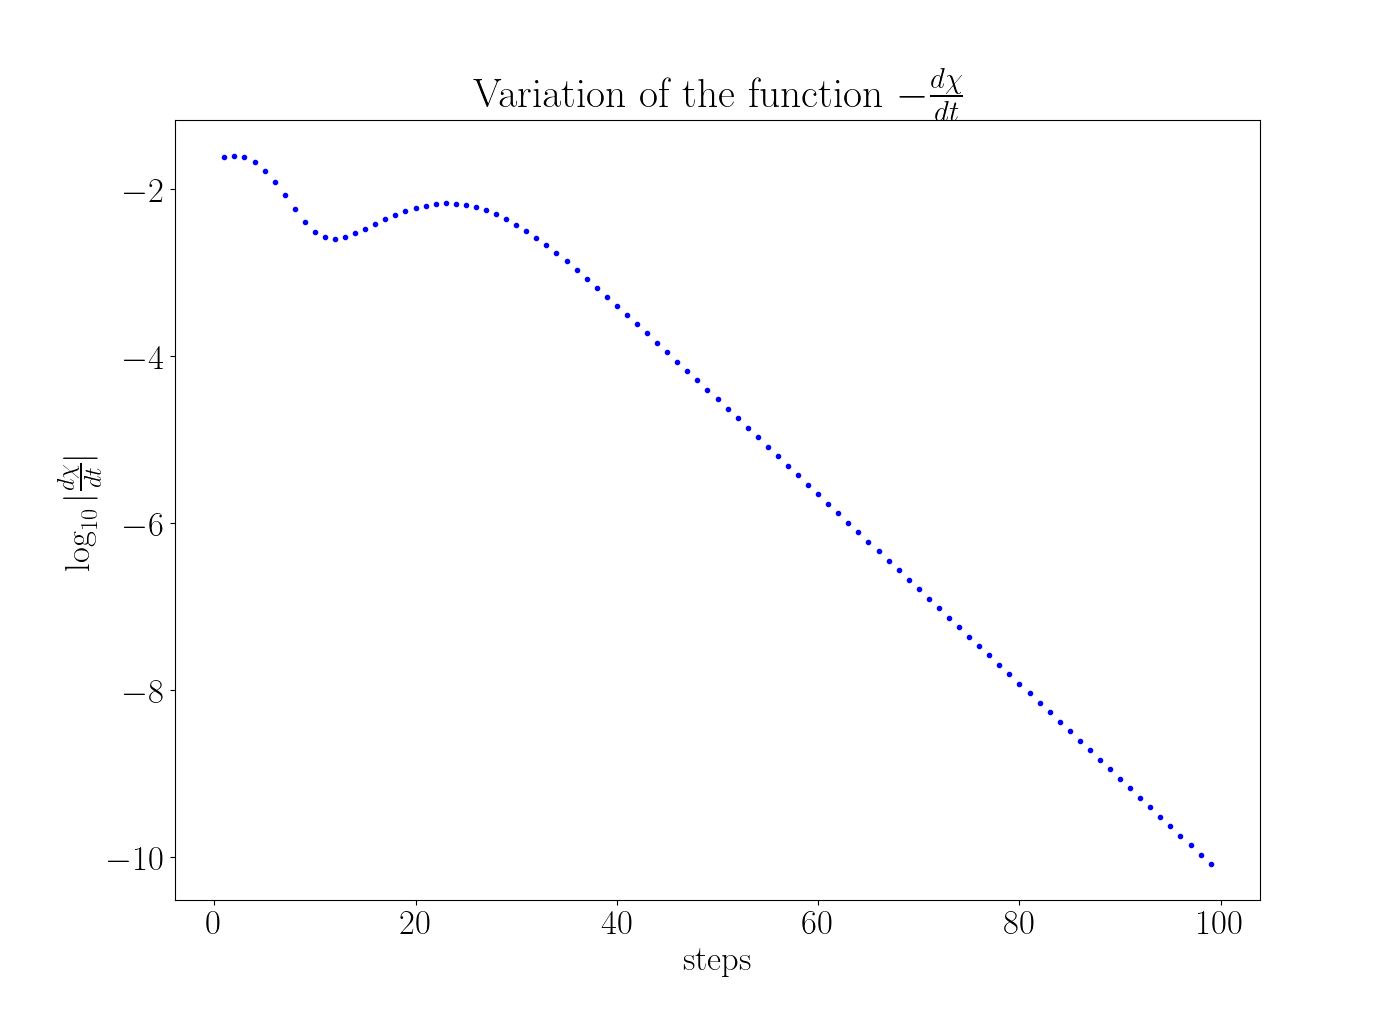
\includegraphics[scale=0.37]{../figures/Svsi.png}
	\captionof{figure}{Variation of the function \( \frac{\:\mathrm{d}\chi}{\:\mathrm{d}t}\) for an arbitrary choice of \(A\) and \(C\). The flow of \(A\) towards a diagonal form is clear.}
\end{center}
The double bracket flow
\begin{equation}\begin{aligned}
	\frac{\:\mathrm{d}A}{\:\mathrm{d}t} = \left[  \left[ A, C \right], A  \right] 
\end{aligned}\end{equation}
is thus a flow towards the minima of the function \( \chi = \text{tr}\left( \left( A - C \right) ^2 \right)  \) .
\subsection{Double-Bracket flow as a descent equation}
The double-bracket flow equation for a symmetric matrix also arises naturally as the equation of motion of a matrix \(X\) (in the space of \(X \in Q X_0 Q^T\)) along that path which minimizes the function
\begin{equation}\begin{aligned}
	f(X) =  ||X - P(X)||^2
\end{aligned}\end{equation}
That is, starting with a matrix \(X_0\) and a transformation \(P\) which takes \(X\) to a subspace \( {P(X)}\), we have a family of matrices \(X(Q) = Q^T X_0 Q\) parameterise by the similarity transformation \(Q\), and we want to find the \(X^*\) (and hence the \(U^*\)) which is closest to the above mentioned subspace. If we choose \(P(X) = \text{diag}(X)\), this is like finding the similarity transformation which takes \(X\) closest to its diagonal form. 
\pb Choosing \(P(X) = N\) where \(N\) is diagonal and identifying \(X_0\) as a Hamiltonian \(H\), the function can be written as
\begin{equation}\begin{aligned}
	f(Q) = ||Q^T H Q - N ||^2
\end{aligned}\end{equation}
The norm-squared is defined as
\begin{equation}\begin{aligned}
	f(Q) = \langle \left(Q^T H Q - N\right) \left(Q^T H Q - N\right)\rangle = \text{Tr}\left[\left(Q^T H Q - N\right)^T \left(Q^T H Q - N\right)\right]
\end{aligned}\end{equation}
which means that the function to minimize is
\begin{equation}\begin{aligned}
	f(Q) = \text{Tr}\left[ H^2 \right] + \text{Tr}\left[ N^2 \right] - 2\text{Tr}\left[ Q^THQN \right] \sim - 2\text{Tr}\left[ Q^THQN \right]
\end{aligned}\end{equation}
where we used \(H^T = H, N^T = N\) and ignored the \(Q-\)independent terms at the final step. Expanding \(Q\) in a Taylor-series about \(Q_0\) gives
\begin{equation}\begin{aligned}
	Q = Q_0 e^\delta = Q_0 + Q_0 \delta + Q_0 \frac{\delta^2}{2} + ..
\end{aligned}\end{equation}
where, in order to make \(Q\) orthogonal, we must have \(\delta = -\delta^T\). The variation on \(F\), upto first order, is then
\begin{equation}\begin{aligned}
	\Delta f(Q_0) &= f(Q_0(1+\delta)) - f(Q_0)\\
		      &= - 2\text{Tr}\left[\left(1-\delta\right)Q^T_0HQ_0\left(1+\delta\right)N \right] + 2\text{Tr}\left[ Q_0^THQ_0N \right]\\
		      &= 2\text{Tr}\left[\delta Q_0^T H Q_0 N \right] - 2\text{Tr}\left[Q^T_0 HQ_0\delta N \right]\\
		      &= 2\text{Tr}\left[Q_0^T H Q_0 N Q_0^T Q\delta\right] - 2\text{Tr}\left[ N Q^T_0 HQ_0\delta\right]\\
		      &= 2\text{Tr}\left[\left(Q_0 N Q_0^T H Q_0 - H Q_0 N\right)^T Q_0 \delta\right]\\
		      &= 2\langle Q_0 N Q_0^T H Q_0 - H Q_0 N, Q_0 \delta\rangle\\
	\implies \nabla f(Q) \cdot Q\delta &= 2\langle Q_0 N Q_0^T H Q_0 - H Q_0 N, Q_0 \delta\rangle\\
	\implies \nabla f(Q) &= Q_0 N Q_0^T H Q_0 - H Q_0 N
\end{aligned}\end{equation}
Since a descent equation is defined as \(\dot x = -\nabla f(x)\), the equation for \(Q\) is 
\begin{equation}\begin{aligned}
	\dot Q = H Q N - Q N Q^T H Q
\end{aligned}\end{equation}
Defining a family of similarity-connected Hamiltonians \(H(Q) = Q^T H_0 Q\) (we have relabelled \(H\) as \(H_0\)), the equation for \(Q\) can be written as
\begin{equation}\begin{aligned}
	\dot Q = H_0 Q N - Q N Q^T H_0 Q = Q H N - Q N H = Q \left[ H, N \right] 
\end{aligned}\end{equation}
And the gradient equation in terms of \(H\) is
\begin{equation}\begin{aligned}
	\dot H = \dot{Q^T}H_0 Q + Q^T H_0 \dot Q =  \left[ N, H \right] Q^T H_0 Q +  Q^T H_0 Q \left[ H, N \right] = \left[ N, H \right] H -  H \left[ N, H \right]\\
	= \left[\left[ N, H \right], H\right] 
\end{aligned}\end{equation}
This is identical to the double-bracket flow equation \ref{dbflow}, with the indetification \(A = H\) and \(C = -N\). We thus see that starting from the equation of motion along the path of steepest descent of a function \(f(Q)\) in the space of orthogonal matrices, we end up with exactly the same double bracket flow equation. The function that we are minimizing (\(f(Q)\)), in terms of \(H(Q)\), is 
\begin{equation}\begin{aligned}
	g(H(Q)) = \text{Tr}\left[ H^2 \right] + \text{Tr}\left[ N^2 \right] - 2\text{Tr}\left[ Q^THQN \right] = \text{Tr}\left[ H^2 + N^2  - 2 H N \right] 
\end{aligned}\end{equation}
which is identical to the function in eq.~\ref{minfunc}.

\subsection{URG as a double-bracket flow}
The difference RG equation for URG can be written in the form
\begin{equation}
	\Delta \mathcal{H} (\omega,D) =  \left[\left[ \mathcal{H}^d, \frac{1}{\omega_1 - \omega_0}G\mathcal{H}^I\right],\mathcal{H}\right] - \ham^I\\
\end{equation}
Assuming a fixed point is reached, the URG equation acts as an optimizer - it minimizes the function
\begin{equation}
\chi_j = \bra{\Psi^i_{j^*}}\left(\mathcal{H}^I_j\right)^2\ket{\Psi^i_{j^*}}
\end{equation}
The definition of this function and the explanation of the symbols requires that a UV-IR scheme be defined. We can order the energy of the electrons as \(\epsilon_1 < \epsilon_2 < ... < \epsilon_j < ... < \epsilon_N\). The URG scheme consists of sequentially decoupling the states \(\epsilon_N\), then \(\epsilon_{N-1}\), and so on. At the \(j^\text{th}\) step, the Hamiltonian can be partitioned in the subspace of the electron being decoupled; the partitioning looks like
\begin{equation}
	\mathcal{H}^0_j + c_j^\dagger T_j + T_j^\dagger c_j
\end{equation}
\(\mathcal{H}^0_j\) is the part that \textit{does not} scatter between \(\ket{\hat n_j} = 0,1\), while \(\mathcal{H}^I_j = c_j^\dagger T_j + T_j^\dagger c_j\) is the part that \textit{does} scatter between states with a definite value of \(\hat n_j\). If, at some value of \(j\) which we call \(j^*\), the denominator of the Green's function in \(\Delta \ham\) vanishes, we call this a fixed point. From the discussion in subsection \ref{match}, we know that if we split \(\ket{\Psi_{j^*}}\) as \(\ket{\Psi_{j^*}} =\ket{\Psi^1_{j^*}}+\ket{\Psi^0_{j^*}}\), then at the fixed point we will have \(\ham^I \ket{\Psi^i_{j^*}} = 0\) for \(i\) either 0 or 1. We define \(i\) to be that component which vanishes at the fixed point. This completes the definition of \(\ket{\Psi^i_{j^*}}\).
\pb The first observation that we will make is that \(\chi_j\) is semi-positive definite. This is because it can be expressed as the norm-squared of a state vector.
\begin{equation}
	\chi_j = \bra{\Psi^i_{j^*}}\left(\mathcal{H}^I_j\right)^2\ket{\Psi^i_{j^*}} = \langle\phi | \phi \rangle \geq 0, \left[\text{where }\ket{\phi} = \mathcal{H}^I_j\ket{\Psi^i_{j^*}}\right]
\end{equation}
The difference equation for \(\chi_j\) is
\begin{equation}\begin{aligned}
	\Delta \chi_j = 2\bra{\Psi^i_{j^*}}\mathcal{H}^I_j\Delta \mathcal{H}^I_j \ket{\Psi^i_{j^*}}= 2\bra{\Psi^i_{j^*}}\mathcal{H}^I_j\left(\mathcal{H}^I_{j-1} - \mathcal{H}^I_j\right)\ket{\Psi^i_{j^*}}\\
\end{aligned}\end{equation}
The first part of the inner product is zero. To see why, note that from the nature of URG, once \(j\) has been decoupled, it is diagonal in all the subsequent Hamiltonians. Hence, \(\mathcal{H}_{j-1}^I\) will be diagonal in \(j\), while \(\mathcal{H}_j^I\) is, by definition, off-diagonal in \(j\). The product \(\mathcal{H}_j^I\mathcal{H}_{j-1}^I\) will hence be off-diagonal and will change \(\hat n_j\). Hence, it will vanish when taken inside an inner product.
\pb What remains is
\begin{equation}\begin{aligned}
	\Delta \chi_j = -2\bra{\Psi^i_{j^*}}\left(\mathcal{H}^I_j\right)^2\ket{\Psi^i_{j^*}} = -2 \chi_j\leq 0\\
\end{aligned}\end{equation}
At the fixed point \(j^*\) of URG, \(\ham^I \ket{\Psi^i_{j^*}} = 0\), so \(\Delta \chi_{j^*} = 0\).
Combining the three points:
\begin{equation}\begin{aligned}
\chi_j \geq 0, && \Delta \chi_j \leq 0, && \Delta \chi_{j^*} = 0
\end{aligned}\end{equation}
we can say that URG starts from a non-minimal value of \(\chi\) and flows to its minimum \(\chi^* = 0\) at the fixed point. 
\pb However, the difficulty with such a function definition is that it depends on a particular state \(\ket{\Psi_{j^*}}\) which we do not know \textit{a prior}. For a more universal definition, we can work with
\begin{equation}\begin{aligned}
	\Gamma_j = \text{Tr}\left[\left(\mathcal{H}^I_j\right)^2\right]
\end{aligned}\end{equation}
This function is also positive semi-definite (because it is a sum of inner products), and its derivative is always negative meaning it monotonically decreases (can be proved exactly as we proved it for \(\chi_j\)), but it is not necessary that it will be 0 at the fixed point. If the choice of URG \(\omega\) is one such that at the fixed point, the interaction coupling vanishes, then \(\Gamma_j\) will vanish and it will have flown to its minima. Otherwise, it will stop at a non-zero value, which can be considered to be  its minima, given that particular value of \(\omega\).
\pb This minimization (for \(\Gamma_j(\omega)\)) has been demonstrated numerically in fig.~\ref{minim}, where URG has been performed on a very simple model of potential scatter:
\begin{equation}
	\mathcal{H} = \sum_k \epsilon_k \hat n_k + J \sum_{k \neq k^\prime} c^\dagger_k c_{k^\prime}
\end{equation}
\begin{center}
	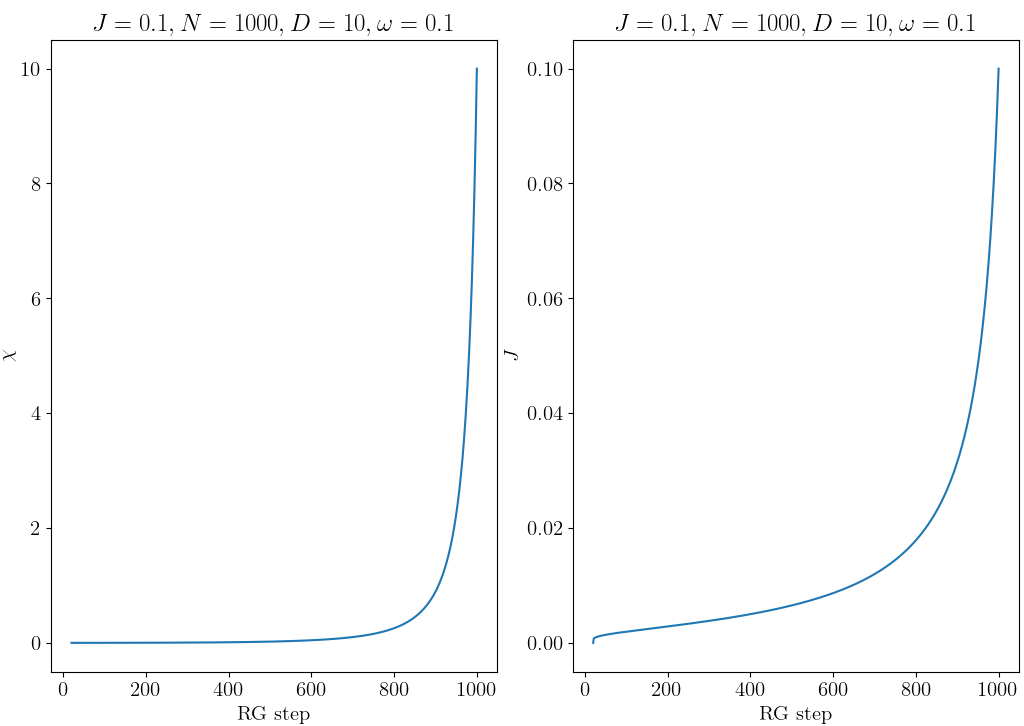
\includegraphics[scale=0.6]{../figures/pot_scatt_dbrack.png}
	\captionof{figure}{Variation of $J$ and $\chi$ for the potential scattering problem.}
	\label{minim}
\end{center}
}


\comm{
We can also obtain the Friedel sum rule from here. The number of electrons before adding the impurity is
\begin{equation}\begin{aligned}
	N^0  = \oint \frac{dz}{2\pi i}n_F(z) \frac{\partial{}}{\partial{z}} \ln \text{Det} \left\{G^{-1}_{c0}(z)\right\}
\end{aligned}\end{equation}
The number of electrons after adding the impurity is
\begin{equation}\begin{aligned}
	N  = \oint \frac{dz}{2\pi i}n_F(z) \left[\frac{\partial{}}{\partial{z}} \ln \text{Det} \left\{G^{-1}_d(z)\right\} + \frac{\partial{}}{\partial{z}} \ln \text{Det} \left\{G^{-1}_{c0}(z)\right\} \right]
\end{aligned}\end{equation}
The change is
\begin{equation}\begin{aligned}
	\Delta N &= \oint \frac{dz}{2\pi i}n_F(z) \frac{\partial{}}{\partial{z}} \ln \text{Det} \left\{G^{-1}_d(z)\right\}\\
		 &= \oint \frac{dz}{2\pi i}n_F(z) \frac{\partial{}}{\partial{z}} \ln \left\{\text{Det} G_d(z)\right\}^{-1}\\
		 &= -\oint \frac{dz}{2\pi i}n_F(z) \frac{\partial{}}{\partial{z}} \ln \left\{\text{Det} G_d(z)\right\}\\
		 &= -\oint \frac{dz}{2\pi i}n_F(z) \frac{\partial{}}{\partial{z}} \ln \left\{\text{Det} G_d(z)\right\}\\
\end{aligned}\end{equation}
	At the FO fixed point, \(G_d\) looks like
\begin{equation}\begin{aligned}
	G_d = \frac{1}{\omega - \epsilon_d}
\end{aligned}\end{equation}
which is a pole at \(\epsilon_d\). Also, at this fixed point, \(\epsilon_d=0\) so that the pole is actually at the FS. Since there are no zeros, we can write
\begin{equation}\begin{aligned}
	n_{\text{Det }G_d^{-1}(\Gamma_0)}\vert_\text{FO} = 1
\end{aligned}\end{equation}
At the SC fixed point, the Green's function takes the general form. However, we have the following expressions for the real and imaginary parts of the self-energy
\begin{equation}\begin{aligned}
\Sigma(z) = \frac{\Delta}{\pi}\ln \left| \frac{z + D}{z - D} \right| - i\Delta
\end{aligned}\end{equation}
Close to the Fermi surface (\(z \to 0\)), the real part drops out. We can therefore write
\begin{equation}\begin{aligned}
	G_d(z) &= \frac{1}{z - \epsilon_d - i\Delta}, &&\forall z \in \Gamma_0\\
	       &=\frac{\frac{1}{\Delta}}{ \frac{z - \epsilon_d}{\Delta} - i}
\end{aligned}\end{equation}
For a thermodynamically large system, \(\Delta \to \infty\), which means the numerator now becomes zero, while the denominator becomes \(-i\)(non-zero). This means, we have one zero and no poles:
\begin{equation}\begin{aligned}
	n_{\text{Det }G_d^{-1}(\Gamma_0)}\vert_\text{SC} = -1
\end{aligned}\end{equation}
}

\comm{
	The impurity-Green's function for such a Hamiltonian is
\begin{equation}\begin{aligned}
	G_{dd}^\sigma = \lim_{\eta \to 0}\bra{d\sigma}\frac{1}{\omega - \ham_\text{high-T, imp} + i \eta} \ket{d\sigma} = \lim_{\eta \to 0}\frac{1}{\omega - \epsilon_d + i\eta}
\end{aligned}\end{equation}
This Green's function has only a real pole, so the state will be infinitely long-lived, signaled by a Dirac-delta density of states:
\begin{equation}\begin{aligned}
	\rho = -\frac{1}{\pi}\text{Im}G_{dd}^\sigma = \delta \left( \omega - \epsilon_d \right) 
\end{aligned}\end{equation}
\textbf{This means that the electron on the impurity will always be localised, and will not be able to tunnel into the conduction band, thereby adding no state to the Fermi volume.}
\begin{equation}\begin{aligned}
	\frac{\mathcal{V}}{\left( 2\pi \right) ^3}\left(\text{Fermi volume}\right) = \frac{V}{\left( 2\pi \right) ^3}v_F = N_{CB}
\end{aligned}\end{equation}
where \(N_{CB}\) is the number (per spin) of conduction electrons and \(\mathcal{V}\) is the real space volume. At the low temperature strong-coupling fixed point, we have \(\epsilon_d^* = -\frac{U^*}{2} = 0\), so the effective Hamiltonian is
\begin{equation}\begin{aligned}
	\ham_\text{low-T} = \sum_{k\sigma}\epsilon_k \hat n_{k\sigma} + v\sum_{\sigma}\left(c^\dagger_{1\sigma}c_{2\sigma} + \text{h.c.} \right) + j\vec{S_1}\cdot\vec{S_2} + k \vec{C_1}\cdot\vec{C_2}
\end{aligned}\end{equation}
Since we are in the first quadrant, we will have \(j \gg k\). Also, we typically have \(v \sim 10 j\) such that we can keep just the \(v\) as a first approximation.
\begin{equation}\begin{aligned}
	\ham_\text{low-T} = \sum_{k\sigma}\epsilon_k \hat n_{k\sigma} + v\sum_{\sigma}\left(c^\dagger_{1\sigma}c_{2\sigma} + \text{h.c.} \right)
\end{aligned}\end{equation}
This is a \textit{resonant level model} with zero onsite energy. The site-diagonal Greens function is
\begin{equation}\begin{aligned}
	G_{dd}^\sigma = \lim_{\eta \to 0}\frac{1}{\omega -\Sigma + i\eta }
\end{aligned}\end{equation}
where \(\Sigma\) is the (complex) self-energy of the impurity site induced by virtual fluctuations into the conduction bath. We can split that into a real and an imaginary part \(\Sigma = \Sigma_0 - i\Delta\), where \(\Delta \sim \rho V^2\). Since the self-energy has an imaginary part, the poles of the Green's function will now be complex, and the states will have a finite lifetime, which is encoded in the fact that the dirac delta dos now broadens into a Lorentzian :
\begin{equation}\begin{aligned}
	\rho (\omega) = \frac{1}{\pi}\frac{\Delta}{\left( \omega - \Sigma_0 \right) ^2 + \Delta^2}
\end{aligned}\end{equation}
\textbf{Since this impurity state is delocalised over long time scales compared to \(\tau \sim \frac{1}{\Delta}\), it gets added to the Fermi volume.} The total number of states added will be the impurity occupancy \(n_d\), which can be calculated from the d.o.s. 
\begin{equation}\begin{aligned}
	n_d = 2\int_{-\infty}^0 \frac{1}{\pi}\frac{\Delta}{\left(\omega - \Sigma_0 \right)^2 + \Delta^2} = \frac{2}{\pi} \cot^{-1} \left(\frac{\Sigma_0}{\Delta} \right)
\end{aligned}\end{equation}
The factor of 2 is the spin-degeneracy. At the strong-coupling fixed point, we have \(V \gg 1 \implies \Delta \gg 1 \implies n_d \approx 1\). The Luttinger sum becomes
\begin{equation}\begin{aligned}
	\frac{V}{\left( 2\pi \right) ^3}v_F = N_{CB} + 1
\end{aligned}\end{equation}
This single-occupancy also constrains the phase shift \(\delta(\epsilon_F)\) suffered by the conduction electrons at the Fermi surface as they scatter off the impurity site; from Friedel's sum rule, we can write
\begin{equation}\begin{aligned}
	\frac{2}{\pi}\delta(\epsilon_F) = \Delta N_L
\end{aligned}\end{equation}
where \(\Delta N_L\) is the change in Luttinger's volume. For this case, it is 1. The phase shift is thus
%
\begin{equation}\begin{aligned}
	\delta(\epsilon_F) = \frac{\pi}{2}
\end{aligned}\end{equation}
The change in Luttinger's number also allows us to calculate the Wilson ratio of the system, from eq.~\ref{wilson_luttinger}.
\begin{equation}\begin{aligned}
	R = 1 + \sin^2 \left( \frac{\pi}{2}\Delta N_L \right) = 1 + \sin^2 \frac{\pi}{2} = 2
\end{aligned}\end{equation}
}

\comm{
\begin{gather}
 \eta^\dagger = \fr{1}{\omega - H_e \hat n_q}c^\dagger_q T,\;\;\;\;\;\;\; \eta = \fr{1}{\omega - H_h (1-\hat n_q)}T^\dagger c_q
 \end{gather}
 Then,
 \beq
 \implies& \fr{1}{\omega - H_e \hat n_q}c^\dagger_q T= c^\dagger_qT\fr{1}{\omega - H_h (1-\hat n_q)}\\
 \implies& c_q^\dagger T H_h(1-\hat n_q) = H_e \hat n_q c_q^\dagger T\\
 \implies& \fr{1}{\omega - H_e \hat n_q}c_q^\dagger T H_h(1-\hat n_q) = \fr{1}{\omega - H_e \hat n_q}H_e \hat n_q c_q^\dagger T\\
 \implies& \eta^\dagger H_h(1-\hat n_q) = H_e \hat n_q \fr{1}{\omega - H_e \hat n_q}c_q^\dagger T\\
 \implies& \eta^\dagger H_h(1-\hat n_q) = H_e \hat n_q \eta^\dagger\\
 \implies& \eta^\dagger H_h = H_e \hat \eta^\dagger\label{iden}
\eeq
Using this identity and its conjugate (\il{\eta H_e = H_h \hat \eta}), the expression for \il{\eta H \eta^\dagger} can be simplified:
\beq
 \eta \ham \eta^\dagger &= \eta H_e \hat n_q \eta^\dagger\\
                &= H_h \eta \eta^\dagger\\
                &= H_h (1-\hat n_q)
\eeq
Similarly,
\beq
 \eta^\dagger  \ham \eta&= \eta^\dagger  H_h \eta\\
                & = H_e \eta^\dagger \eta\\
                &= H_e \hat n_q
\eeq
Also, 
\beq
\ham\eta - \ham\eta^\dagger + \eta^\dagger \ham - \eta\ham = \rr{\eta^\dagger_q H_h - H_e \eta^\dagger} + \rr{H_h \eta - \eta H_e} + \eta^\dagger T^\dagger c_q - \eta c^\dagger_q T + \\
c_q^\dagger T \eta - T^\dagger c_q \eta^\dagger
\eeq
By virtue of eq.~\ref{iden} and its conjugate, the first two terms will vanish, so we are left with
\beq[link]
\ham\eta - \ham\eta^\dagger + \eta^\dagger \ham - \eta\ham = \eta^\dagger T^\dagger c_q - \eta c^\dagger_q T + c_q^\dagger T \eta - T^\dagger c_q \eta^\dagger
\eeq
From eqs.~\ref{id1} and \ref{id2},
\begin{gather}
\eta^\dagger T ^\dagger c_q = \eta^\dagger \eta c_q^\dagger T \eta = \hat n_q c_q^\dagger T\eta = c_q^\dagger T\eta\\
T ^\dagger c_q \eta^\dagger = \eta c_q^\dagger T \eta \eta^\dagger = \eta c_q^\dagger T \rr{1-\hat n_q} = \eta c_q^\dagger T\\
\end{gather}
Eq.~\ref{link} becomes
\beq
 \ham\eta - \ham\eta^\dagger + \eta^\dagger \ham - \eta\ham &= c_q^\dagger T\eta - \eta c^\dagger_q T + c_q^\dagger T \eta - \eta c_q^\dagger T
                                     &=2\qq{c_q^\dagger T,\eta}
\eeq
}

\comm{
To begin, we choose an electron with a particular value of quantum numbers, which we label \(q\). It might be the electron with the highest momentum or that at the first lattice site. The goal is to obtain a unitary transformation \il{U_q} that diagonalizes this Hamiltonian in this particular electron's basis. Once this is done, we can choose another electron (the next highest momentum or the second lattice site) and diagonalize the Hamiltonian in this electron's basis.
\pb \(U_q\) is defined by
\beq
\tilde \ham = U_q \ham U^\dagger_q \text{   such that  } \qq{\tilde \ham,n_q} = 0
\eeq
Another way to express the above problem is that, with the original Hamiltonian \il{\ham}, the diagonal terms are not zero:
\beq
n_q \ham(1-n_q) \neq 0
\eeq
so we want to find a rotated Hamiltonian \il{\tilde \ham = U_q \ham U_q^\dagger} such that the off-diagonal term is zero:
\beq[solve]
n_q \tilde \ham(1-n_q) =0
\eeq
To make progress, we write the Hamiltonian \il{\ham} as
\beq[ham]
\ham = \ham^D + \ham^I + \ham^i 
\eeq
\begin{minipage}{300pt}
    \il{\ham^D} is the diagonal part of the Hamiltonian, something of the form \il{\sum_k \epsilon_k n_k}.
It also has the self energies that might arise from certain interactions.
For example, if we have an interaction term of the form \(J \sum_{k_1,k_2}c^\dagger_{k_1}c_{k_2}\), the term where both momenta are equal gives a diagonal term \(J c^\dagger_{k_1}c_{k_1}\).
Such terms are also included in \(\ham^D\).
\pb \il{\ham^I} is the interaction between the current degree of freedom \il{q} and the remaining degrees of freedom \(k\).
It will consist of terms like \il{c^\dagger_q c_k} or \il{c^\dagger_k c_q} that scatter between the current degree of freedom and the other degrees of freedom.
\end{minipage}
\begin{minipage}{165pt}
\begin{center}
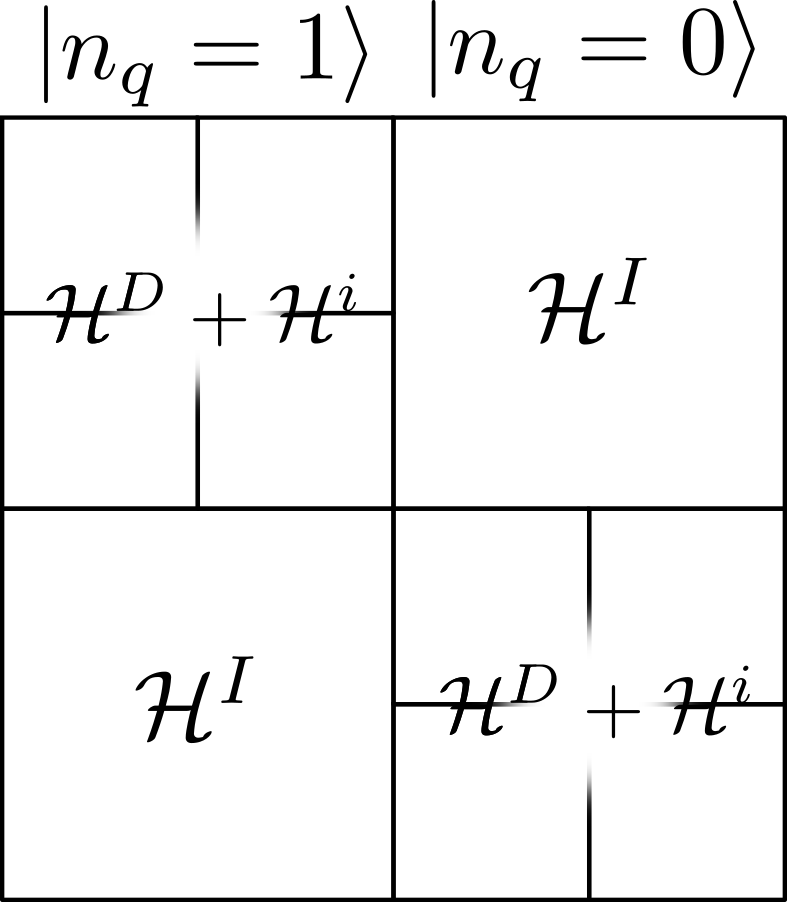
\includegraphics[scale=0.6]{ham.png}
\captionof{figure}{Block-decomposition of Hamiltonian}
\end{center}
\end{minipage}
\pb The third term \il{\ham^i} has interactions between the remaining degrees of freedom.
This term will also be diagonal in \il{n_k} because it doesn't involve scattering either from or into \il{q} states.
It will involve terms like \il{c^\dagger_{k_1}c_{k_2}}.
\pb Let \(\cc{\ket{\Psi}_q}\) be the set of states in which \(\ham\) assumes a diagonal form in the space of \(q\). This diagonal form is of course also what we get when we apply the unitary transformation \(U_q\) on the Hamiltonian.
\beq[tanjiro]
\ham \ket{\Psi}_q = \tilde \ham \ket{\Psi}_q
\eeq
\comm{
    To find the form for \il{U_k}, we define a few things.
First,
\beq
P_k = U_k^\dagger n_k U_k
\eeq
To get a feel for what \il{P_k} is, note that
\beq
\qq{\ham, P_k} = \qq{U^\dagger_k U_k \ham, U_k^\dagger n_k U_k} = U_k^\dagger \qq{\wl \ham, n_k}U_k = 0
\eeq
\il{P_k} is hence those degrees of freedom in which the given Hamiltonian \il{\ham} is diagonal.
Hence it is natural that they are obtained by rotating the \il{n_k}.
If we were to go to the eigenbasis of \ham, the form for \il{\wl \ham} will be 
\beq
\begin{pmatrix} E_1 & \\ & E_2 \end{pmatrix}
\eeq
while the form for \il{P_k} will be
\beq
\begin{pmatrix} 1 & 0  \\ 0 & 0\end{pmatrix}
\eeq
It is obvious that
\beq
P_k^2 = P_k
\eeq
Another thing that we will define is
\beq
\ol \ham  = P_k \ham P_k
\eeq
\il{\ol \ham} is a matrix that, in the eigenbasis of \ham, has only the upper diagonal block of \il{\ham}.
 That is, you first form a matrix by keeping only the upper diagonal block of \il{\wl \ham} and then rotating to the basis of \il{n_k}.
Finally, let \il{\psi} be a wavefunction such that
\beq
P\psi = \psi
\eeq
This means that \il{\psi} is an eigenvector of \il{P_k} and hence also of \il{\ham} since \il{P_k} and \il{\ham} commute.
\\\\
Combining \il{P_k \ham = \ham P_k} and the idempotence of \il{P_k} gives
\beq
\ham P_k = P_k \ham = P_k \ham P_k = \ol\ham
\eeq
Operating this equation on \il{\psi} gives
\beq[tanjiro]
\ham \psi = \ol \ham \psi
\eeq
}
This is the equation we will use to find \il{U_q}.
But first we will write \il{\psi} in the following fashion:
\beq
\ket{\Psi} = a_1 \ket{1,\Psi_1} + a_0\ket{0,\Psi_0}
\eeq
In the kets \(\ket{1,\Psi_1}\) and \(\ket{0,\Psi_0}\), the first entry (\(0/1\)) signifies whether the degree of freedom \il{q} is occupied or not, and the second entry is the wavefunction of the remaining degrees of freedom.
This is just a resolution of the total wavefunction in the two-dimensional Hilbert space of \il{q}.
\comm{
The Hamiltonian \il{\ol\ham} can also be decomposed in a similar form.
Note however that since it is already diagonal in \il{n_k}, it won't have any scattering in \il{k}, and hence won't have a term like \il{\ham^I}.
\beq
\ol \ham = \ol \ham^D + \ol \ham^i
\eeq}
Substituting the decomposition of \il{\ket{\Psi}} and \(\ham\) into eq.~\ref{tanjiro} gives
\beq[zenitsu]
\tilde \ham \rr{a_1\ket{1,\Psi_1} + a_0\ket{0,\Psi_0}} = \qq{\ham^D  + \ham^I + \ham^i }\rr{a_1 \ket{1,\Psi_1} + a_0\ket{0,\Psi_0}}
\eeq
To get expressions from this, note that on the left hand side, \il{\tilde \ham} does not scatter \il{q}, so it will not change the left entry in the kets; it can only change the right entries.
Similarly, on the right hand side, \il{\ham^D} and \il{\ham^i} will not change the occupation of the \il{k} degree of freedom.
\il{\ham^I} however \it{will} change it.
Matching the states with \il{\ket{0}} gives
\beq
\tilde \ham a_0\ket{0,\Psi_0} = \rr{\ham^D + \ham^i}a_0\ket{0,\Psi_0} + \ham^Ia_1\ket{1,\Psi_1}
\eeq
We can simplify this equation by noting that
\begin{gather}
\ham^D = \text{ Tr} \qq{\ham^D \hat n_q}\hat n_q + \text{ Tr} \qq{\ham^D (1 - \hat n_q)}(1-\hat n_q)\\
 \implies  \ham^D \ket{0,\psi_0} = \text{ Tr} \qq{\ham^D (1 - \hat n_q)}(1-\hat n_q)\ket{0,\psi_0}
\end{gather}
and
\begin{gather}
 \ham^I = \text{ Tr} \qq{c^\dagger_q \ham } c_q + c^\dagger_q \text{ Tr} \qq{\ham c_q}
 \implies \ham^I\ket{1,\psi_1} = \text{ Tr} \qq{c^\dagger_q \ham } c_q \ket{1,\psi_1}
\end{gather}
Substituting these in the equation gives
\begin{gather}
\tilde \ham a_0\ket{0,\Psi_0} = \cc{\text{ Tr} \qq{\ham^D (1 - \hat n_q)}(1-\hat n_q) + \ham^i}a_0\ket{0,\Psi_0}
+ \text{ Tr} \qq{c^\dagger_q \ham } c_q a_1\ket{1,\Psi_1}\\
\implies \cc{\tilde\ham - \ham^i - \text{ Tr} \qq{\ham^D (1 - \hat n_q)}(1-\hat n_q)} a_0 \ket{0,\Psi_0}
= \text{ Tr} \qq{c^\dagger_q \ham } c_q a_1\ket{1,\Psi_1}
\end{gather}
Defining \il{\hat \omega = \tilde\ham - \ham^i}, we get the result
\beq
a_0 \ket{0,\Psi_0} = \qq{\hat \omega - \text{ Tr} \qq{\ham^D (1 - \hat n_q)}(1-\hat n_q)}^{-1}\text{ Tr} \qq{c^\dagger_q \ham } c_q a_1\ket{1,\Psi_1}
\eeq
We define 
\beq[etadef]
\eta_q \equiv \fr{1}{\hat \omega - \text{ Tr} \qq{\ham^D (1 - \hat n_q)}(1-\hat n_q)}\text{ Tr} \qq{c^\dagger_q \ham } c_q
\eeq
which gives the equation a compact form
\beq
a_0 \ket{0,\Psi_0} = \eta_q a_1\ket{1,\Psi_1}
\eeq
The equation obtained by matching the states \il{\ket{1}} is
\beq
a_1 \ol \ham \ket{1,\Psi_1} &= \rr{\ham^D + \ham^i}a_1\ket{1,\Psi_1} + \ham^I a_0\ket{0,\Psi_0}\\
                &= \rr{\text{ Tr }\qq{\ham^D \hat n_q}\hat n_q + \ham^i}a_1\ket{1,\Psi_1} + c^\dagger_q \text{ Tr }\qq{\ham c_q}a_0\ket{0,\Psi_0}\\
\implies a_1 \ket{\Psi_1} &= \rr{\ol\ham - \ham^i - \text{ Tr }\qq{\ham^D \hat n_q}\hat n_q }^{-1} c^\dagger_q \text{ Tr }\qq{\ham c_q}a_0\ket{0,\Psi_0}\\
              &=\mu_q a_0\ket{0,\Psi_0}
\eeq
where 
\beq[etadagdef]
\mu_q = \fr{1}{\hat \omega - \text{ Tr} \qq{\ham^D \hat n_q}\hat n_q} c_q^\dagger \text{ Tr}\qq{ \ham c_q}
\eeq
We thus get the following two equations:
\begin{gather}
    a_0 \ket{0,\Psi_0} = \eta_q a_1\ket{1,\Psi_1}\label{eta}\\
    a_1 \ket{1,\Psi_1} = \mu_q a_0\ket{0,\Psi_0}\label{etad}
\end{gather}
Combining eqs.~\ref{eta} and \ref{etad}, we get
\beq
a_0 \ket{0,\Psi_0} = \eta_q a_1\ket{1,\Psi_1} = \eta_q \mu_q a_0 \ket{0,\Psi_0}
\eeq
Combining this with the fact that \il{\mu_q} should have a \il{c^\dagger_q} and hence should give \il{\mu_q \ket{1,\Psi_1}}, we get
\beq
\eta_q \mu_q = 1 - \hat n_q
\eeq
Similarly, combining the equations the other way round gives
\beq[prod]
\mu_q \eta_q = \hat n_q
\eeq
As a consequence,
\beq
 \cc{\eta_q,\mu_q} &= 1\\
 \qq{\eta_q,\mu_q} &= 1 - 2\hat n_q\\
\eeq
Other properties include
\begin{gather}
\eta_q^2 = \rr{\mu_q}^2 = 0\\
\hat n_q \eta_q = (1-\hat n_q)\mu_q = 0\\
\eta_q \hat n_q=\eta_q\\
\mu_q(1-\hat n_q) = \mu_q
\end{gather}
We now need to find the unitary operation \il{U_q} that disentangles the state \il{\ket{1,\Psi_1}} from the state \il{\ket{\Psi}}.
For the sake of unitarity, we restrict \(\mu_q = \eta^\dagger_q\). This restriction is transferred to the values of \(\hat \omega\).
Using eq.~\ref{eta},
\beq
\ket{\Psi} = a_1\ket{1,\Psi_1} + a_0\ket{0,\Psi_0}  = a_1\ket{1,\Psi_1} +  \eta_q a_1\ket{1,\Psi_1} = \rr{1+\eta_q}\ket{1,\Psi_1}
\eeq
Since \(\eta^2 = 0\), we can write \(1+\eta_q = e^{\eta_q}\). \(S \equiv e^{\eta_q}\) constitutes a similarity transformation. It is shown in ref.~\cite{suzuki} that corresponding to a similarity transformation \(e^\omega\),there exists a unitary transformation \(e^G\) where
\beq
G = \tanh^{-1}\rr{\omega - \omega^\dagger}
\eeq
Applying that to the problem at hand gives
\beq
 U^\dagger &= \ex{\tanh^{-1}\rr{\eta - \eta^\dagger}}\\
       &= \frac{1 + \eta - \eta^\dagger}{1 + \cc{\eta,\eta^\dagger}}\\
       &= \fr{1}{\sqrt 2}\rr{1 + \eta - \eta^\dagger}
\eeq
The unitary operator that transforms the entangled eigenstate \il{\ket{\Psi}} to the eigenstate with good quantum number \il{n_q}, \il{\ket{1,\Psi_1}} is thus
\beq
U_q = \fr{1}{\sqrt 2}\rr{1 + \eta_q^\dagger - \eta_q}
\eeq
It can also be written as \(\ex{\frac{\pi}{4}\rr{\eta^\dagger_q - \eta_q}}\) because
\beq
 \ex{\frac{\pi}{4}\rr{\eta^\dagger_q - \eta_q}} &= 1 + \rr{\eta^\dagger_q - \eta_q}\fr{\pi}{4} + \frac{1}{2!}\rr{\eta^\dagger_q - \eta_q}^2\rr{\fr{\pi}{4}}^2 + \frac{1}{3!}\rr{\eta^\dagger_q - \eta_q}^3\rr{\fr{\pi}{4}}^3 + ...\\
&= 1 + \rr{\eta^\dagger_q - \eta_q}\fr{\pi}{4} - \frac{1}{2!}\rr{\fr{\pi}{4}}^2 - \frac{1}{3!}\rr{\eta^\dagger_q - \eta_q}\rr{\fr{\pi}{4}}^3 + \frac{1}{4!}\rr{\fr{\pi}{4}}^4 + ...\\
&= \cos \frac{\pi}{4} + \rr{\eta^\dagger_q - \eta_q}\sin\fr{\pi}{4}\\
&= 1 + \eta_q^\dagger - \eta_q
\eeq
There we used
\beq
\rr{\eta^\dagger_q - \eta_q}^2 = {\eta^\dagger_q}^2 + \eta_q^2 - \cc{\eta^\dagger_q,\eta_q} = -1 &&\qq{\because\eta^2 = {\eta^\dagger}^2=0}
\eeq
and so
\beq
\rr{\eta^\dagger_q - \eta_q}^3 = -1\rr{\eta^\dagger_q - \eta_q}
\eeq
and so on.

\pb The form of the rotated Hamiltonian can now be written down.
\beq[roth]
 \wl\ham &= U_q \ham U_q^\dagger\\
     &= \hf\rr{1+\eta_q^\dagger - \eta_q}\ham\rr{1 + \eta_q - \eta^\dagger_q}\\
                &= \hf\rr{1+\eta_q^\dagger - \eta_q}\rr{\ham + \ham\eta - \ham\eta_q^\dagger}\\
                &=\hf\rr{\ham+ \ham\eta - \ham\eta_q^\dagger + \eta_q^\dagger \ham + \eta_q^\dagger\ham\eta_q - \eta_q^\dagger \ham\eta_q^\dagger - \eta_q\ham - \eta_q \ham \eta_q + \eta_q \ham \eta_q^\dagger}\\
&=\hf\rr{\ham^D + \ham^i + \ham^I + \ham\eta - \ham\eta_q^\dagger + \eta_q^\dagger \ham + \eta_q^\dagger\ham\eta_q - \eta_q^\dagger \ham\eta_q^\dagger - \eta_q\ham - \eta_q \ham \eta_q + \eta_q \ham \eta_q^\dagger}\\
&=\hf\rr{\ham^D + \ham^i + \ham^I + \qq{\eta^\dagger_q - \eta,\ham} + \eta_q^\dagger\ham\eta_q - \eta_q^\dagger \ham\eta_q^\dagger - \eta_q \ham \eta_q + \eta_q \ham \eta_q^\dagger}\\
\eeq
In the last step I split \il{\ham} using eq.~\ref{ham}.
\beq[ham]
\ham = \ham^D + \ham^I + \ham^i 
\eeq
\il{\ham^D} is the diagonal part of the Hamiltonian, something of the form \il{\sum_k \epsilon_k n_k}.
It also has the self energies that might arise from certain interactions.
For example, if we have an interaction term of the form \(J \sum_{k_1,k_2}c^\dagger_{k_1}c_{k_2}\), the term where both momenta are equal gives a diagonal term \(J c^\dagger_{k_1}c_{k_1}\).
Such terms are also included in \(\ham^D\).
\pb \il{\ham^I} is the interaction between the current degree of freedom \il{q} and the remaining degrees of freedom \(k\).
It will consist of terms like \il{c^\dagger_q c_k} or \il{c^\dagger_k c_q} that scatter between the current degree of freedom and the other degrees of freedom.
\pb The third term \il{\ham^i} has interactions between the remaining degrees of freedom.
This term will also be diagonal in \il{n_k} because it doesn't involve scattering either from or into \il{q} states.
It will involve terms like \il{c^\dagger_{k_1}c_{k_2}}.
\pb For reasons that will become apparent later, we will split the terms into two groups:
\beq
 \tilde \ham &= \hf\rr{\underbrace{\ham^D + \ham^i + \qq{\eta^\dagger_q - \eta,\ham} + \eta_q^\dagger\ham\eta_q + \eta_q \ham \eta_q^\dagger}_\text{group 1} + \overbrace{\ham^I - \eta_q^\dagger \ham\eta_q^\dagger - \eta_q \ham \eta_q}^\text{group 2}}\\
\eeq
Group 2 consists of purely off-diagonal terms; they amount to 0. To see how, note that terms that have two \il{\eta_k} or two \il{\eta_q^\dagger} can only be nonzero if the intervening \il{\ham} has a creation or destruction operator.
We resolve the Hamiltonian in the basis of \il{q} in the following form:
\beq[hisoka]
 \ham &= \text{Tr}\qq{\ham \hat n_q}\hat n_q + \text{Tr}\qq{\ham \rr{1 - \hat n_q}}\rr{1 - \hat n_q} + c_q^\dagger \text{Tr}\qq{\ham c_q} + \text{Tr}\qq{c_q^\dagger \ham}c_q\\
      &=H_e \hat n_q + H_h (1-\hat n_q) + c^\dagger_q T + T^\dagger c_q
\eeq
Using this form, we can write
\beq[beats]
\eta_q \ham \eta_q = \eta_q c_q^\dagger  T \eta_q
\eeq
and
\beq[tora]
\eta_q^\dagger \ham\eta_q^\dagger = \eta_q^\dagger T^\dagger c_q \eta_q^\dagger
\eeq
We can also write the off-diagonal part as
\beq
\ham^I = c^\dagger_q T + T^\dagger c_q
\eeq
Group 2 becomes
\beq
\text{group 2} = c^\dagger_q T + T^\dagger c_q - \eta_q^\dagger T^\dagger c_q \eta_q^\dagger - \eta_q c_q^\dagger  T \eta_q
\eeq
To simplify this, we use the definition of \(\eta^\dagger_q\), eq.~\ref{etadagdef}, to write \(\eta_q\):
\beq
\eta_q = \rr{\eta_q^\dagger}^\dagger = \text{ Tr}\qq{ c^\dagger_q\ham }c_q\fr{1}{\hat \omega - \text{ Tr} \qq{\ham^D \hat n_q}\hat n_q} = T^\dagger c_q \fr{1}{\hat \omega - H_e \hat n_q}
\eeq
Using this, we can write
\beq
 \eta_q c_q^\dagger  T \eta_q &= T^\dagger c_q \fr{1}{\hat \omega - H_e \hat n_q}c_q^\dagger  T \eta_q\\
                  &= T^\dagger c_q \rr{\fr{1}{\hat \omega - H_e \hat n_q}c_q^\dagger  T} \eta_q\\
                  &= T^\dagger c_q \eta_q^\dagger\eta_q &&\qq{\text{eq.~\ref{etadagdef}}}\\
                  &= T^\dagger c_q \hat n_q &&\qq{\text{eq.~\ref{antic}}}
\eeq
which gives
\beq[id1]
 \eta_q c_q^\dagger  T \eta_q  &= T^\dagger c_q 
\eeq
Similarly, we can express \(\eta^\dagger_q\) by taking Hermitian conjugate of \(\eta_q\):
\beq
\eta^\dagger_q = \fr{1}{\hat \omega - H_h \rr{1 - \hat n_q}}T^\dagger c_q 
\eeq
which gives
\beq[id2]
\eta_q^\dagger T^\dagger c_q \eta_q^\dagger = c_q^\dagger T
\eeq
Substituting the expressions \ref{id1} and \ref{id2}, we get \(\text{group 2}=0\).
Substituting this in the rotated Hamiltonian gives
\beq
\wl \ham = \hf\rr{\ham^D + \ham^i + \ham\eta - \ham\eta_q^\dagger + \eta_q^\dagger \ham + \eta_q^\dagger\ham\eta_q - \eta_q\ham  + \eta_q \ham \eta_q^\dagger}
\eeq
To simplify the last 6 terms, we note the following:
\begin{gather}
 \eta_q^\dagger = \fr{1}{\omega - H_e \hat n_q}c^\dagger_q T,\;\;\;\;\;\;\; \eta_q = \fr{1}{\omega - H_h (1-\hat n_q)}T^\dagger c_q
 \end{gather}
 Then,
 \beq
 \implies& \fr{1}{\omega - H_e \hat n_q}c^\dagger_q T= c^\dagger_qT\fr{1}{\omega - H_h (1-\hat n_q)}\\
 \implies& c_q^\dagger T H_h(1-\hat n_q) = H_e \hat n_q c_q^\dagger T\\
 \implies& \fr{1}{\omega - H_e \hat n_q}c_q^\dagger T H_h(1-\hat n_q) = \fr{1}{\omega - H_e \hat n_q}H_e \hat n_q c_q^\dagger T\\
 \implies& \eta_q^\dagger H_h(1-\hat n_q) = H_e \hat n_q \fr{1}{\omega - H_e \hat n_q}c_q^\dagger T\\
 \implies& \eta_q^\dagger H_h(1-\hat n_q) = H_e \hat n_q \eta_q^\dagger\\
 \implies& \eta_q^\dagger H_h = H_e \hat \eta_q^\dagger\label{iden}
\eeq
Using this identity and its conjugate (\il{\eta_q H_e = H_h \hat \eta_q}), the expression for \il{\eta_q H \eta_q^\dagger} can be simplified:
\beq
 \eta_q \ham \eta_q^\dagger &= \eta_q H_e \hat n_q \eta_q^\dagger\\
                &= H_h \eta_q \eta_q^\dagger\\
                &= H_h (1-\hat n_q)
\eeq
Similarly,
\beq
 \eta_q^\dagger  \ham \eta_q&= \eta_q^\dagger  H_h \eta_q\\
                & = H_e \eta_q^\dagger \eta_q\\
                &= H_e \hat n_q
\eeq
Also, 
\beq
\ham\eta - \ham\eta_q^\dagger + \eta_q^\dagger \ham - \eta_q\ham = \rr{\eta^\dagger_q H_h - H_e \eta_q^\dagger} + \rr{H_h \eta - \eta H_e} + \eta_q^\dagger T^\dagger c_q - \eta_q c^\dagger_q T + \\
c_q^\dagger T \eta_q - T^\dagger c_q \eta_q^\dagger
\eeq
By virtue of eq.~\ref{iden} and its conjugate, the first two terms will vanish, so we are left with
\beq[link]
\ham\eta - \ham\eta_q^\dagger + \eta_q^\dagger \ham - \eta_q\ham = \eta_q^\dagger T^\dagger c_q - \eta_q c^\dagger_q T + c_q^\dagger T \eta_q - T^\dagger c_q \eta_q^\dagger
\eeq
From eqs.~\ref{id1} and \ref{id2},
\begin{gather}
\eta_q^\dagger T ^\dagger c_q = \eta_q^\dagger \eta_q c_q^\dagger T \eta_q = \hat n_q c_q^\dagger T\eta_q = c_q^\dagger T\eta_q\\
T ^\dagger c_q \eta_q^\dagger = \eta_q c_q^\dagger T \eta_q \eta_q^\dagger = \eta_q c_q^\dagger T \rr{1-\hat n_q} = \eta_q c_q^\dagger T\\
\end{gather}
Eq.~\ref{link} becomes
\beq
 \ham\eta - \ham\eta_q^\dagger + \eta_q^\dagger \ham - \eta_q\ham &= c_q^\dagger T\eta_q - \eta_q c^\dagger_q T + c_q^\dagger T \eta_q - \eta_q c_q^\dagger T
                                     &=2\qq{c_q^\dagger T,\eta_q}
\eeq
Putting it all together,
\beq
 \wl \ham &= \hf\rr{\ham^D + \ham^i + \ham\eta - \ham\eta_q^\dagger + \eta_q^\dagger \ham + \eta_q^\dagger\ham\eta_q - \eta_q\ham  + \eta_q \ham \eta_q^\dagger}\\
      &=\hf\rr{\ham^D + \ham^i} + \qq{c_q^\dagger T,\eta_q} + \hf\qq{H_e \hat n_q + H_h(1-\hat n_q)}
\eeq
}
\comm{
One further simplification is possible.
The last two terms constitute the total diagonal part of the Hamiltonian, but so do the first two terms:
\beq
\ham^D + \ham^i = H_e \hat n_q + H_h\rr{1-\hat n_q}
\eeq
Hence,
\beq
 \wl \ham &= \hf\rr{\ham^D + \ham^i + \ham\eta - \ham\eta_q^\dagger + \eta_q^\dagger \ham + \eta_q^\dagger\ham\eta_q - \eta_q\ham  + \eta_q \ham \eta_q^\dagger}\\
      &=H_e \hat n_q + H_h(1-\hat n_q) + \qq{c_q^\dagger T,\eta_q}\\
      &=\text{Tr}\qq{\ham\hat n_q}\hat n_q + \text{Tr}\qq{\ham\hat(1- n_q)}(1-\hat n_q) + \qq{c_q^\dagger \text{Tr}\rr{\ham c_q},\eta_q}
\eeq
The two terms at the front can be written in a slightly different fashion.
\beq
 \text{Tr}\qq{\ham\hat n_q}\hat n_q + \text{Tr}\qq{\ham(1- \hat n_q)}(1-\hat n_q) &= \text{Tr}\qq{\ham\hat n_q}\hat n_q + \text{Tr}\qq{\ham(\hat n_q -1)}(\hat n_q -1)\\
                                          &=\text{Tr}\qq{\ham\hat n_q}\hat n_q + \text{Tr}\qq{\ham(\hat n_q -1)}n_q -\text{Tr}\qq{\ham\hat(n_q -1)}\\
                                          &=\text{Tr}\qq{\ham\rr{2\hat n_q - 1}}\hat n_q -\text{Tr}\qq{\ham(\hat n_q -1)}\\
                                          &=\text{Tr}\qq{\ham\rr{\hat n_q - \hf}}2\hat n_q -\text{Tr}\qq{\ham(\hat n_q -\hf)} + \hf\text{Tr}\qq{\ham} \\
                                          &= \text{Tr}\qq{\ham\rr{\hat n_q - \hf}}\rr{2\hat n_q - 1} + \hf\text{Tr}\qq{\ham}\\
                                          &=\text{Tr}\qq{\ham\tau_q}2\tau_q + \hf\text{Tr}\qq{\ham}\\
\eeq
The last term can be written as:
\beq
 \qq{c_q^\dagger \text{Tr}\rr{\ham c_q},\eta_q} &= c_q^\dagger \text{Tr}\rr{\ham c_q}\eta_q - \eta_qc_q^\dagger \text{Tr}\rr{\ham c_q}\\
                        &=\rr{2\hat n_q - 1}c_q^\dagger \text{Tr}\rr{\ham c_q}\eta_q - \rr{1-2\hat n_q}\eta_qc_q^\dagger \text{Tr}\rr{\ham c_q}
\eeq
I used \il{\hat n_q c^\dagger_q = c^\dagger_q} and \il{\hat n_q \eta_q = 0}.
Then,
\beq
 \qq{c_q^\dagger \text{Tr}\rr{\ham c_q},\eta_q} = 2\tau_q \cc{c_q^\dagger \text{Tr}\rr{\ham c_q},\eta_q}
\eeq
The final form of the rotated Hamiltonian is
\beq[final2]
\wl \ham = U_q \ham U_q^\dagger =  \text{Tr}\qq{\ham\hat n_q}\hat n_q + \text{Tr}\qq{\ham(1- \hat n_q)}(1-\hat n_q) + 2\tau_q \cc{c_q^\dagger \text{Tr}\rr{\ham c_q},\eta_q}
\eeq
}

\comm{
	\subsection{Numerical analysis of symmetric Anderson-Kondo (spin) model}
We can look at a special case of the RG equations: \(\epsilon_q = D, \epsilon_d = -\frac{U}{2}, V_0 = V_1, J_z = J_t = \frac{J}{2}\).
\begin{equation}\begin{aligned}
	\Delta U &= \frac{4|V|^2}{\omega - \frac{D}{2} + \frac{U}{2} + \frac{J}{2}} - \frac{4|V|^2}{\omega - \frac{D}{2} - \frac{U}{2} + \frac{J}{4}} - \frac{3J^2}{4}\sum_k \frac{1}{\omega - \frac{D}{2} + \frac{J}{4}}\\
	\Delta V &= -\frac{3J}{4}V\left(\frac{1}{\omega - \frac{D}{2} - \epsilon_d + \frac{J}{2}} + \frac{1}{\omega - \frac{D}{2} + \frac{J}{4}}\right)\\
	\Delta J &= -J^2\frac{1}{\omega - \frac{D}{2} + \frac{J}{4}}\\
\end{aligned}\end{equation}
}
\comm{
For a given set of bare values of the couplings, there are two broad classes of RG flows. The first class is the one in which the Kondo coupling \(J\) flows to a large positive value. These flows are characterized by the condition \(\frac{D}{2} - \omega - \frac{J}{4} > 0\). The fixed point here is the strong-coupling one, in which the impurity spin gets screened from the mobile electrons. The othe class is in which \(J\) flows to zero. This occurs when  \(\frac{D}{2} - \omega - \frac{J}{4} < 0\), and the impurity is decoupled from the mobile electrons in this case. Both class of flows are depicted in figure ~\ref{flows}. The phase diagram is shown in figure ~\ref{phases-siam-kondo}.
\begin{center}
	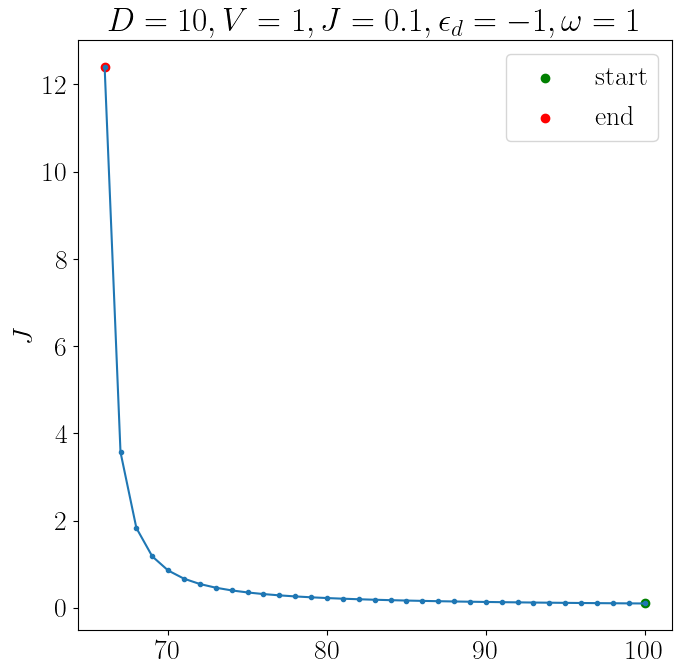
\includegraphics[scale=0.46]{../figures/af.png}
	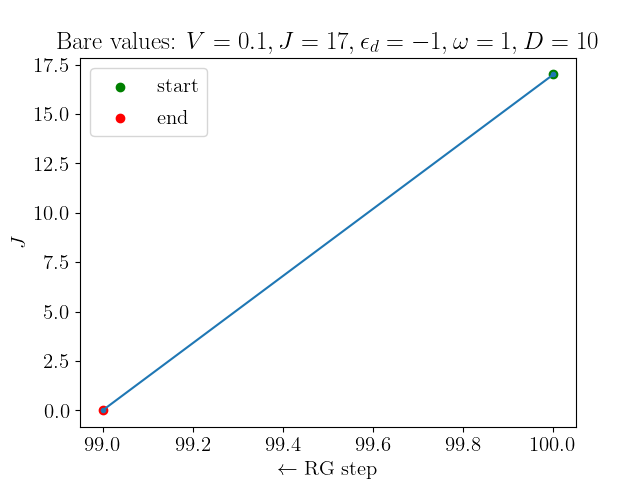
\includegraphics[scale=0.46]{../figures/ferro.png}
	\captionof{figure}{Left: Flow to the strong-coupling fixed point \(J^* > 0\). Right: Flow to the weak-coupling fixed point \(J^* = 0\)}
	\label{flows}
\end{center}
\begin{center}
	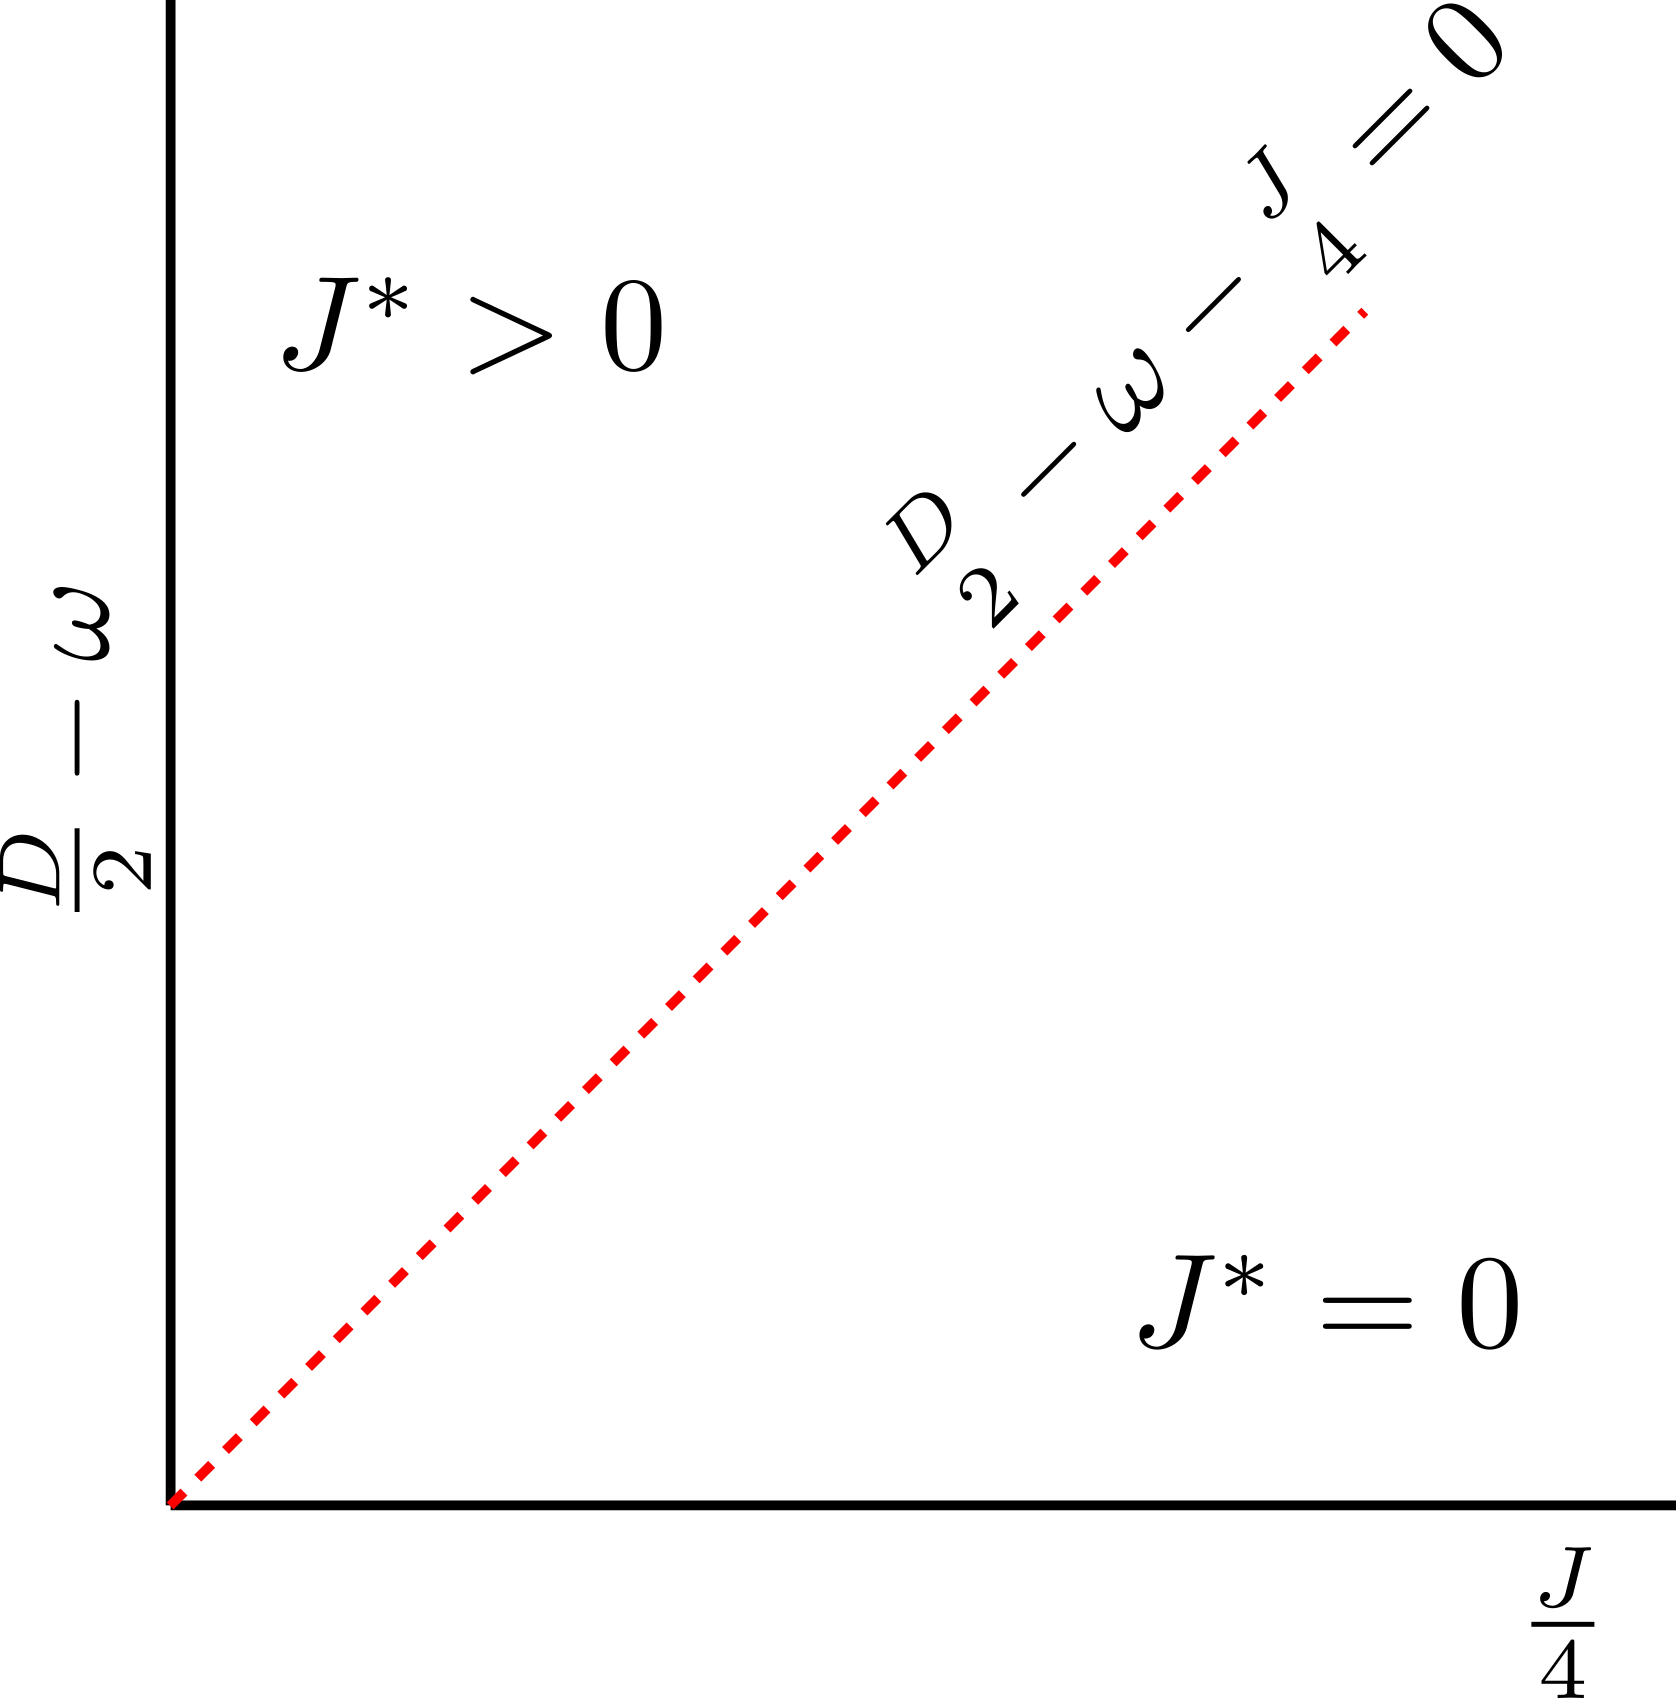
\includegraphics[scale=0.5]{../figures/siam-kondo-phases.png}
\captionof{figure}{Phase diagram for the Anderson-Kondo model, in the \(\frac{D}{2} - \omega\) vs \(\frac{J}{4}\) plane. All quantities involve bare values.}
	\label{phases-siam-kondo}
\end{center}
Within the strong-coupling class of flows, their are two kinds of flows, depending on the behaviour of \(|\epsilon_d|\). If the bare value of \(|\epsilon_d|\) is greater than a certain value (determined by the bare values of \(\omega, D, \text{ and }J\), it will flow to large values. In other words, such a fixed point will be characterized by large \(J\) and large \(|\epsilon_d|\). If we have \(\epsilon_d = -|\epsilon_d|\), such a flow leads to an enhancement of the onsite repulsion \(U\). Such flows are shown in fig.~\ref{flowup}.
\pb If, on the other hand, the bare value of \(|\epsilon_d|\) is lower than a value, it will decay to zero under the RG, resulting in a non-interacting impurity. This is shown in fig.~\ref{flowdown}.
\begin{center}
	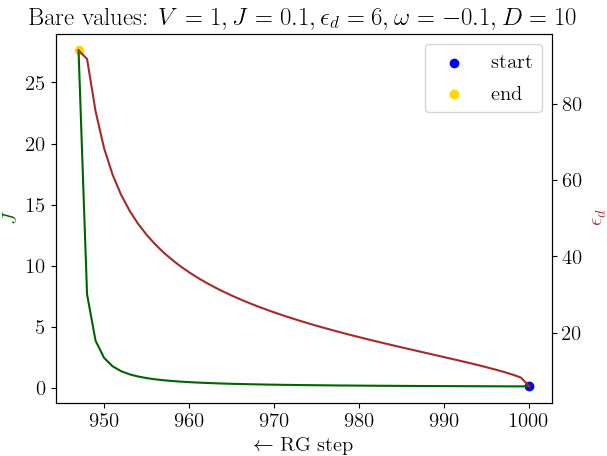
\includegraphics[scale=0.38]{../figures/ed_to_large1.png}
	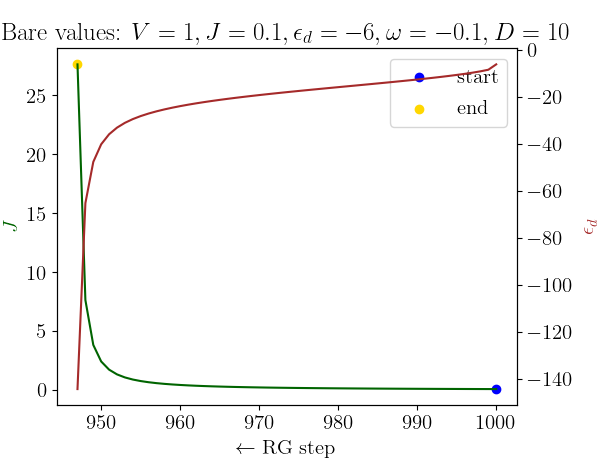
\includegraphics[scale=0.38]{../figures/ed_to_large2.png}
	\captionof{figure}{Flows to large values of \(|\epsilon_d|\), starting from both positive (right) and negative (left) values of \(\epsilon_d\).}
	\label{flowup}
\end{center}
\begin{center}
	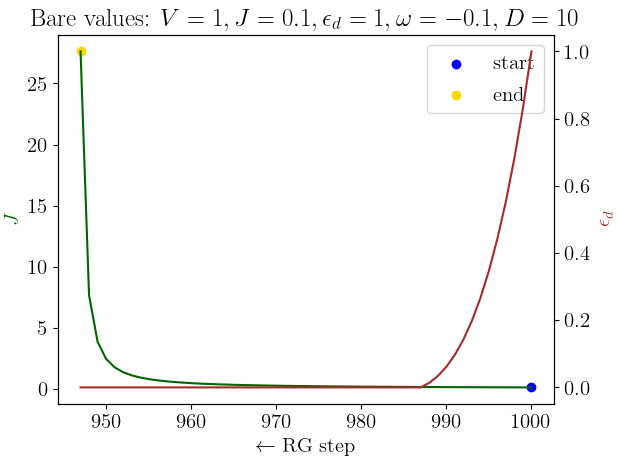
\includegraphics[scale=0.38]{../figures/ed_to_zero1.png}
	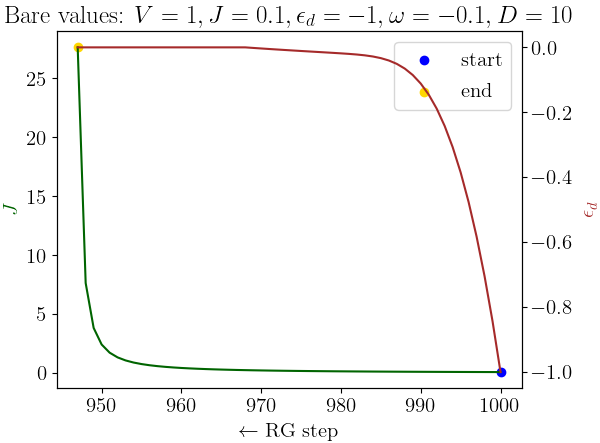
\includegraphics[scale=0.38]{../figures/ed_to_zero2.png}
	\captionof{figure}{Flows in which \(|\epsilon_d|\) decays to zero, starting from both positive (right) and negative (left) values of \(\epsilon_d\).}
	\label{flowdown}
\end{center}
\begin{minipage}{190pt}
The fixed-point value of the Kondo coupling, \(J^*\), is a function of the bare bandwidth we start with. As the bare bandwidth increases, the fixed point value of \(J\) also increases, signalling that in the thermodynamic limit, \(J\) should flow to infinity, see fig.~\ref{JvsD}. This is in line with NRG results which show that for a continuous isotropic dispersion, the Kondo coupling asymptotically flows to infinity as we take larger and larger length scales.
\end{minipage}
\hspace*{20pt}
\begin{minipage}{260pt}
\begin{center}
	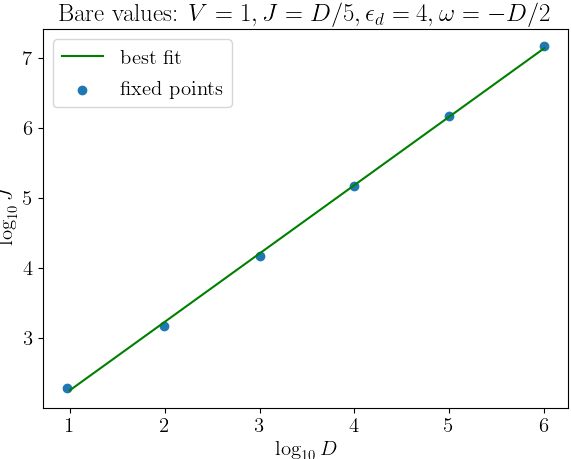
\includegraphics[scale=0.6]{../figures/J_vs_D_finite_w_both_log.png}
	\captionof{figure}{Variation of the fixed point value \(J^*\) against the bare bandwidth \(D\).}
	\label{JvsD}
\end{center}
\end{minipage}
}

\comm{
\subsection{Hole sector}
This will involve terms which start from an empty state (hole). This renormalization is given by 
\beq
T^\dagger c_{q\beta}Gc^\dagger_{q\beta}T
\eeq
where
\begin{flalign*}
&Gc^\dagger_{q\beta}T\\
&= \frac{1}{\omega_0 - \ham_d}\sum_{q\beta}\qq{V_qc^\dagger_{q\beta}c_{d\beta} + K_z \rr{\hat n_d -1}\sum_k c^\dagger_{q\beta}c_{k\beta} + K_t \sum_k c^\dagger_{q\beta}c^\dagger_{k\ol\beta}c_{d\beta}c_{d\ol\beta} }\\
 	     &=\sum_{q\beta}\left[\frac{V_q}{\omega_0 - \hf\epsilon_q - \epsilon_d \hat n_{d\ol\beta} - \frac{1}{2}K_z\rr{\hat n_{d\ol\beta}-1}}c^\dagger_{q\beta}c_{d\beta} + \frac{K_z \rr{\hat n_d -1}}{\omega_0 - \hf\epsilon_q - H_{imp} - \frac{1}{2}K_z\rr{\hat n_{d}-1}}\sum_k c^\dagger_{q\beta}c_{k\beta} \right.\\
 	     &\left.+\frac{K_t }{\omega_0 - \hf\epsilon_q + \frac{1}{2}K_z}\sum_k c^\dagger_{q\beta}c^\dagger_{k\ol\beta}c_{d\beta}c_{d\ol\beta}\right]\\
\end{flalign*}
The renormalization is, therefore,
\begin{flalign*}
	     &\sum_{q\beta}\qq{V_1^*c^\dagger_{d\beta}\hat n_{d\ol\beta}c_{q\beta} + V_0^*c^\dagger_{d\beta}\rr{1 - \hat n_{d\ol\beta}}c_{q\beta} + K_z^+ \hat n_{d\beta}\hat n_{d\ol\beta}\sum_k c^\dagger_{k\beta}c_{q\beta} - K_z^- \left(1 - \hat n_{d\beta}\right)\left(1 - \hat n_{d\ol\beta}\right)\sum_k c^\dagger_{k\beta}c_{q\beta} + K_t \sum_k c^\dagger_{d\beta}c^\dagger_{d\ol\beta}c_{q\beta}c_{k\ol\beta}}Gc^\dagger_{q\beta}T\\
&=\sum_{q\beta}\left[\frac{|V_q|^2 \hat n_{d\beta}\rr{1 - \hat n_{q\beta}}}{\omega_0 - \hf\epsilon_q - \epsilon_d \hat n_{d\ol\beta} - \frac{1}{2}K_z\rr{\hat n_{d\ol\beta}-1}} - \sum_k\frac{V_q^*K_z c^\dagger_{d\beta}c_{k\beta}\rr{1 - \hat n_{d\ol\beta}}\rr{1 - \hat n_{q\beta}}}{\omega_0 - \hf\epsilon_q + \frac{1}{2}K_z} \right.\\
&- \left.\sum_k\frac{V_q^* K_t\hat n_{d\beta}\rr{1 - \hat n_{q\beta}}c^\dagger_{k\ol\beta}c_{d\ol\beta}}{\omega_0 - \hf\epsilon_q + K_z} - \sum_k\frac{K_z V_q\rr{1 - \hat n_{d\ol\beta}}\rr{1 - \hat n_{q\beta}}c^\dagger_{k\beta}c_{d\beta}}{\omega_0 - \hf\epsilon_q + \frac{1}{2}K_z}\right. \\
&+\left. \sum_{kk^\prime}\frac{K_z^2 \rr{1 - \hat n_d}^2\rr{1 - \hat n_{q\beta}}c^\dagger_{k\beta}c_{k^\prime\beta}}{\omega_0 - \hf\epsilon_q - H_{imp} - \frac{1}{2}K_z\rr{\hat n_d - 1}} - \sum_{kk^\prime}\frac{K_z K_t \rr{1 - \hat n_{q\beta}}c^\dagger_{k\beta}c^\dagger_{k^\prime\ol\beta}c_{d\beta}c_{d\ol\beta}}{\omega_0 - \hf\epsilon_q + \frac{1}{2}K_z}\right.\\
&- \left.\sum_k\frac{K_t V_q \rr{1 - \hat n_{q\beta}}\hat n_{d\beta}c^\dagger_{d\ol\beta}c_{k\ol\beta}}{\omega_0 - \hf\epsilon_q + \frac{1}{2}K_z} - \sum_{kk^\prime}\frac{K_z K_t \rr{1 - \hat n_{q\beta}}c^\dagger_{d\beta}c^\dagger_{d\ol\beta}c_{k\beta}c_{k^\prime\ol\beta}}{\omega_0 - \hf\epsilon_q + \frac{1}{2}K_z}\right.\\
&+\left.\sum_{kk^\prime} \frac{K_t^2 \hat n_{d\beta}\hat n_{d\ol\beta}\rr{1 - \hat n_{q\beta}}c_{k^\prime\ol\beta}c^\dagger_{k\ol\beta}}{\omega_0 - \hf\epsilon_q + \frac{1}{2}K_z}\right]
\end{flalign*}
\subsection{Particle sector}
This will involve terms which start from an occupied state (particle). This renormalization is given by 
\beq
c_{q\beta}^\dagger TG T^\dagger c_{q\beta}
\eeq
where
\beq
G T^\dagger c_{q\beta} &= \sum_{q\beta}\frac{1}{\omega - \ham_d}\qq{V_q^*c^\dagger_{d\beta}c_{q\beta} + K_z \rr{\hat n_d -1}\sum_k c^\dagger_{k\beta}c_{q\beta} + K_t \sum_k c^\dagger_{d\beta}c^\dagger_{d\ol\beta}c_{q\beta}c_{k\ol\beta} }\\
			       &=\sum_{q\beta}\left[\frac{V^*_q c^\dagger_{d\beta}c_{q\beta}}{\omega_1 - \hf\epsilon_q - \epsilon_d - \rr{\epsilon_d + U}\hat n_{d\ol\beta} + \frac{1}{2}K_z\hat n_{d\ol\beta}} + \frac{K_z \rr{\hat n_d -1}\sum_k c^\dagger_{k\beta}c_{q\beta}}{\omega_1 - \hf\epsilon_q - H_{imp} + \frac{1}{2}K_z\rr{\hat n_{d}-1}} \right.\\
			       &+\left.\frac{K_t \sum_k c^\dagger_{d\beta}c^\dagger_{d\ol\beta}c_{q\beta}c_{k\ol\beta}}{\omega_1 - \hf\epsilon_q -2\epsilon_d - U + \frac{1}{2}K_z}\right]\\
\eeq
The renormalization is, therefore,
\begin{flalign*}
&\sum_{q\beta}\qq{V_qc^\dagger_{q\beta}c_{d\beta} + K_z \rr{\hat n_d -1}\sum_k c^\dagger_{q\beta}c_{k\beta} + K_t \sum_k c^\dagger_{q\beta}c^\dagger_{k\ol\beta}c_{d\beta}c_{d\ol\beta} }GT^\dagger c_{q\beta}\\
&=\sum_{q\beta}\left[\frac{|V_q|^2 \hat n_{q\beta}\rr{1 - \hat n_{d\beta}}}{\omega_1 - \hf\epsilon_q - \epsilon_d - \left( \epsilon_d + U - \frac{1}{2}K_z \right) \hat n_{d\overline\beta}} - \sum_k\frac{V_qK_z c^\dagger_{k\beta}c_{d\beta}\hat n_{d\ol\beta}\hat n_{q\beta}}{\omega_1 - \hf\epsilon_q - 2\epsilon_d - U + \frac{1}{2}K_z}\right.\\
&-\left. \sum_k\frac{V_q K_t\hat n_{q\beta}\rr{1 - \hat n_{d\beta}}c^\dagger_{d\ol\beta}c_{k\ol\beta}}{\omega_1 - \hf\epsilon_q - 2\epsilon_d - U + \frac{1}{2}K_z} - \sum_k\frac{K_z V_q^*\hat n_{d\ol\beta}\hat n_{q\beta}c^\dagger_{d\beta}c_{k\beta}}{\omega_1 - \hf\epsilon_q -2\epsilon_d - U + \frac{1}{2}K_z} \right.\\
&+\left. \sum_{kk^\prime}\frac{K_z^2 \rr{\hat n_d - 1}^2\hat n_{q\beta}c_{k\beta}c^\dagger_{k^\prime\beta}}{\omega_1 - \hf\epsilon_q - H_{imp} + \frac{1}{2}K_z\rr{\hat n_d - 1}} - \sum_{kk^\prime}\frac{K_z K_t \hat n_{q\beta}c^\dagger_{d\beta}c^\dagger_{d\ol\beta}c_{k\beta}c_{k^\prime\ol\beta}}{\omega_1 - \hf\epsilon_q -2\epsilon_d - U + \frac{1}{2}K_z}\right.\\
&- \left.\sum_k\frac{K_t V^*_q \hat n_{q\beta}\rr{1 - \hat n_{d\beta}}c^\dagger_{k\ol\beta}c_{d\ol\beta}}{\omega_1 - \hf\epsilon_q -2\epsilon_d - U + \frac{1}{2}K_z} - \sum_{kk^\prime}\frac{K_z K_t \hat n_{q\beta}c^\dagger_{k\beta}c^\dagger_{k^\prime\ol\beta}c_{d\beta}c_{d\ol\beta}}{\omega_1 - \frac{1}{2}\epsilon_q - 2\epsilon_q - U + \frac{1}{2}K_z}\right.\\
& +\left. \sum_{kk^\prime}\frac{K_t^2 \left(1 - \hat n_{d\beta}\right) \left(1 - \hat n_{d\ol\beta}\right) \hat n_{q\beta}c^\dagger_{k\ol\beta}c_{k^\prime\ol\beta}}{\omega_1 - \hf\epsilon_q - 2\epsilon_d - U + \frac{1}{2}K_z}\right]
\end{flalign*}
}

\comm{
\subsection{Numerical analysis of symmetric Anderson-Kondo (charge) model}
For the special case of eq.~\ref{symm-charge}, the RG equations simplify to
\begin{equation}\begin{aligned}
	\Delta U &= 4|V|^2\frac{1}{\omega - \frac{D}{2} + \frac{U}{2}} - 4|V|^2\frac{1}{\omega - \frac{D}{2} - \frac{U}{2} + \frac{K}{4}} + \frac{3K^2}{4}\sum_k\frac{1}{\omega - \frac{D}{2} + \frac{K}{4}}\\
	\Delta V &= \frac{V_1 K}{8}\left( \frac{1}{\xi_1} + \frac{1}{\xi_6} \right) \\
	\Delta K &= -\frac{K^2}{4}\frac{1}{\omega - \frac{D}{2} + \frac{K}{4}}
\end{aligned}\end{equation}
}
\comm{
The numerical solutions are identical to the ones obtained in the spin-Kondo, with \(K\) playing the role of \(J\) here.
\begin{center}
	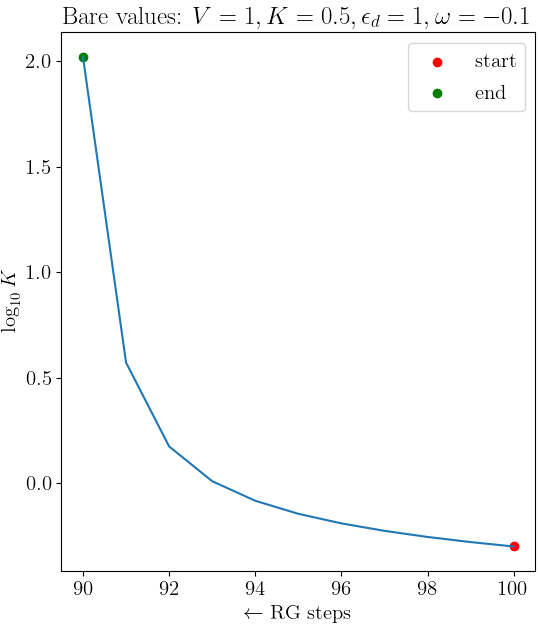
\includegraphics[scale=0.5]{../figures/K_grow.png}
	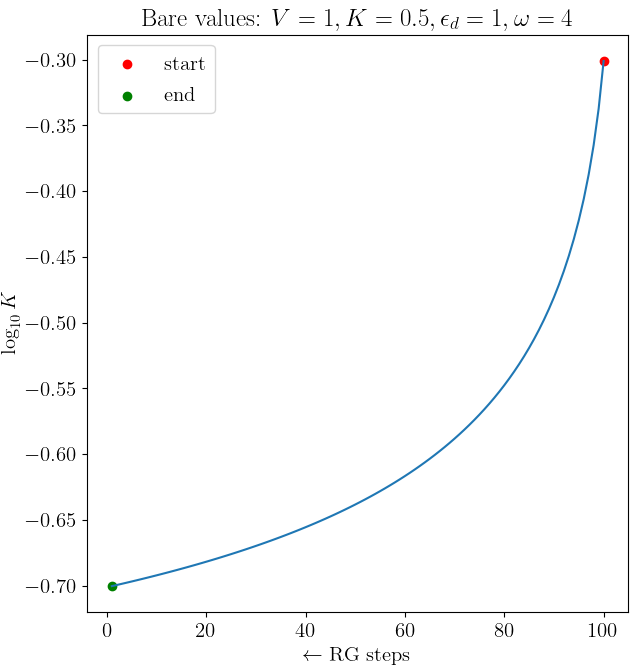
\includegraphics[scale=0.5]{../figures/K_decay.png}
	\captionof{figure}{Flows of the charge-Kondo coupling \(K\) to the strong-coupling fixed point (left) as well as the weak-coupling critical fixed point (right).}
\end{center}
\begin{center}
	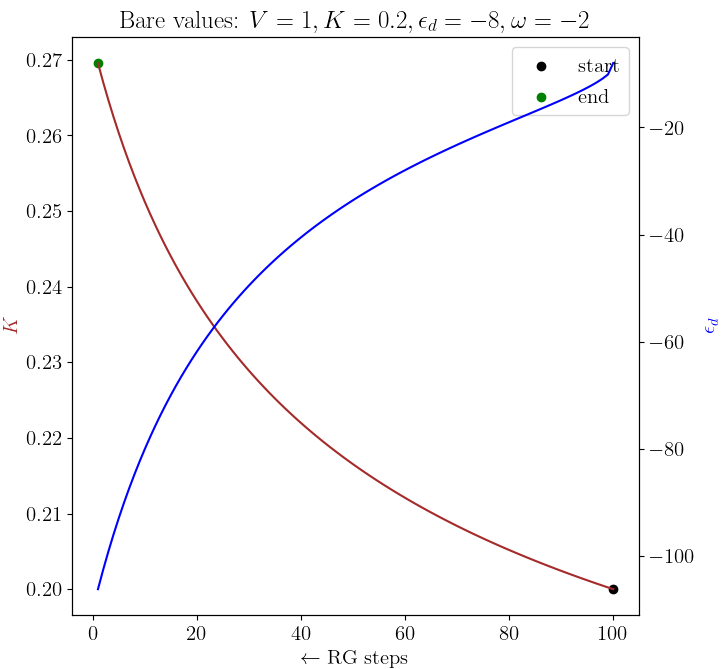
\includegraphics[scale=0.46]{../figures/ed_grow1.png}
	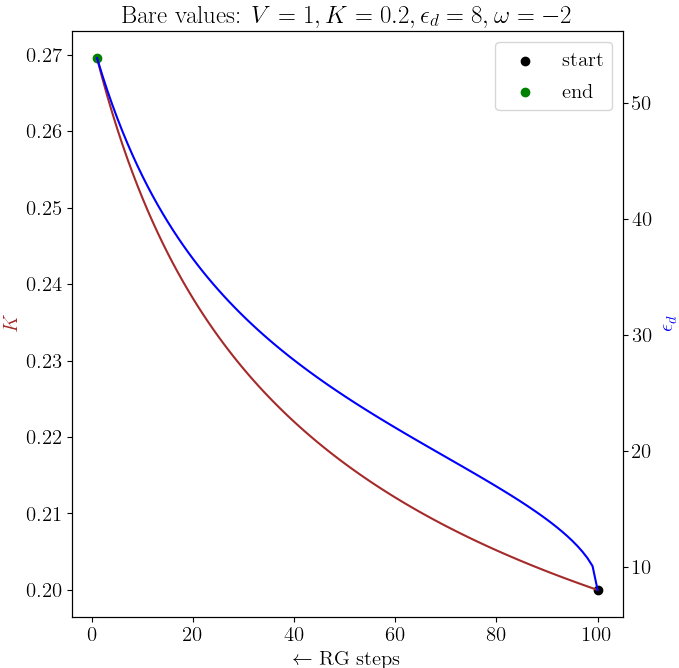
\includegraphics[scale=0.46]{../figures/ed_grow2.png}
	\captionof{figure}{Flow of \(|\epsilon_d|\) to large values, starting from positive (right) and negative values (left). The impurity becomes highly interacting at this fixed point, owing to either a large \(U\) (large repulsion, favouring single occupation) or large \(\epsilon_d\) (large onsite energy, favouring non-single occupation).}
\end{center}
\begin{center}
	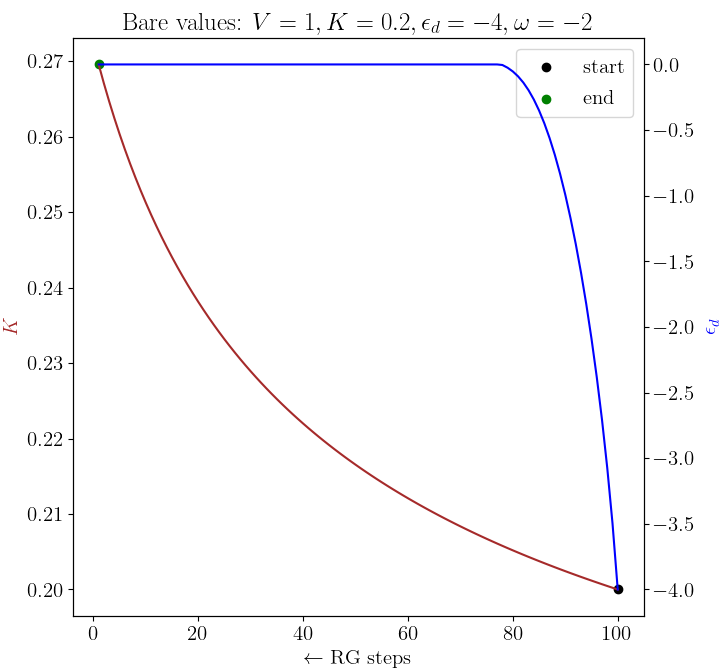
\includegraphics[scale=0.46]{../figures/ed_decay1.png}
	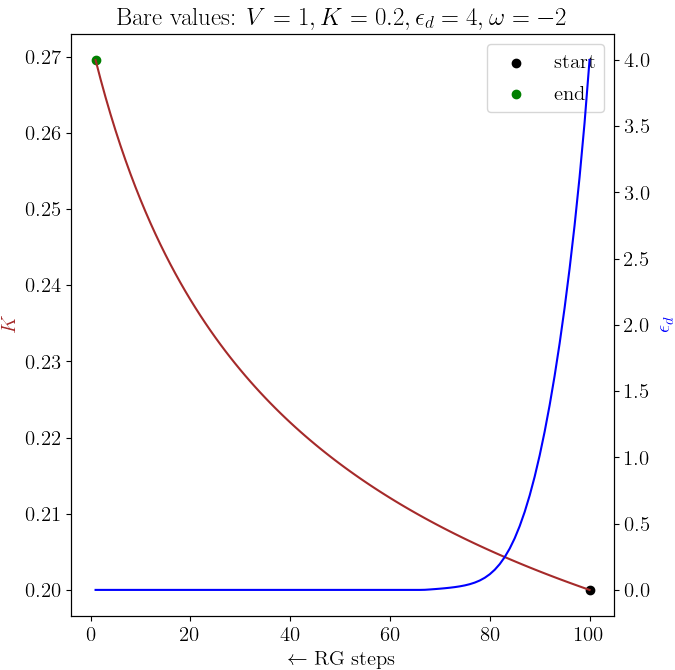
\includegraphics[scale=0.46]{../figures/ed_decay2.png}
	\captionof{figure}{Flow of \(|\epsilon_d|\) to zero, starting from positive (right) and negative values (left). The impurity becomes non-interacting (free orbital) at this fixed point such that all four levels become degenerate in the atomic limit.}
\end{center}
\begin{center}
	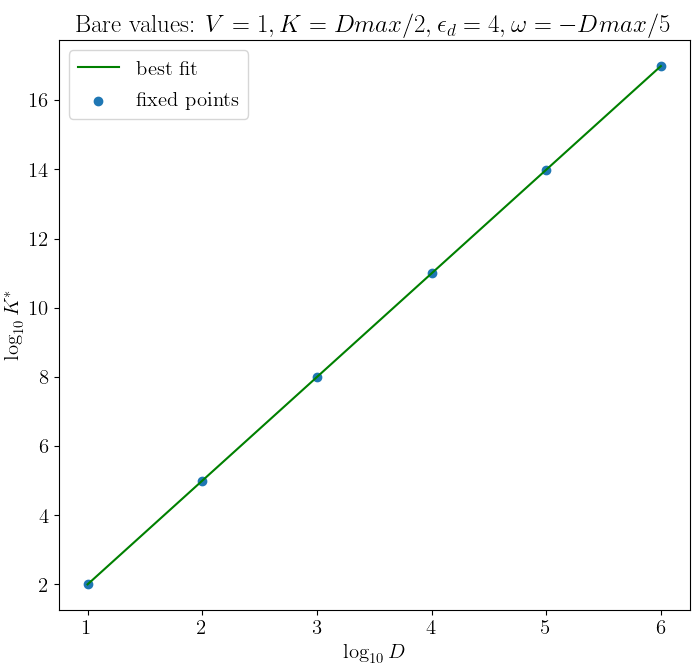
\includegraphics[scale=0.5]{../figures/K_vs_D.png}
	\captionof{figure}{Variation of the fixed-point value of \(K\) with the bare bandwidth, in log scale. Increasing system size (larger \(D\)) results in larger values of \(K^*\).}
\end{center}
}
\comm{
\section{Anderson-Kondo (spin + charge) model URG}
In this section, we will consider the SIAM with both spin and charge fluctuations. This will be a combination of the last two sections. The total Hamiltonian will be
\begin{equation}\begin{aligned}
	\ham =& \sum_{k\sigma}\tau_{k\sigma} + \epsilon_d \hat n_d + U \hat n_{d\uparrow}\hat n_{d \downarrow} + \sum_{k\sigma}\left( V_k c^\dagger_{k\sigma} c_{d\sigma} + \text{h.c.} \right) + J_z S_d^z\sum_{kk^\prime}\left( c^\dagger_{k \uparrow}c_{k^\prime \uparrow} - c^\dagger_{k \downarrow}c_{k^\prime \downarrow} \right) \\
	      &+ J_t \sum_{kk^\prime\sigma}c^\dagger_{d\sigma}c_{d\ol\sigma}c^\dagger_{k\ol\sigma}c_{k^\prime\sigma} + K_z C_d^z \sum_{kk^\prime}\left( c^\dagger_{k\sigma}c_{k^\prime\sigma} - \frac{1}{2}\delta_{kk^\prime} \right) + K_t \sum_{kk^\prime\sigma}\left(c^\dagger_{d\sigma}c^\dagger_{d\ol\sigma}c_{k\ol\sigma}c_{k^\prime\sigma}+\text{h.c.}\right)
\end{aligned}\end{equation}
 There are eight different type of scattering terms:
\begin{equation}\begin{aligned}
	c^\dagger_{q\beta}T_1 &= V_1 c^\dagger_{q\beta}c_{d\beta}\hat n_{d\ol\beta}, &c^\dagger_{q\beta}T_2 &= V_0 c^\dagger_{q\beta}c_{d\beta}\left(1 - \hat n_{d\ol\beta}\right)\\
	c^\dagger_{q\beta}T_3 &= \sum_{k<\Lambda_N}J^z_0 \hat n_{d\beta}\left(1 - \hat n_{d\ol\beta}\right) c^\dagger_{q\beta}c_{k\beta}, &c^\dagger_{q\beta}T_4 &= -\sum_{k<\Lambda_N}J^z_1 \hat n_{d\ol\beta}\left(1 - \hat n_{d\beta}\right) c^\dagger_{q\beta}c_{k\beta}\\
	c^\dagger_{q\beta}T_5 &= \sum_{k<\Lambda_N}J^t c^\dagger_{d\ol\beta}c_{d\beta}c^\dagger_{q\beta}c_{k\ol\beta}, &c^\dagger_{q\beta}T_6 &= K_z^1 \sum_{k<\Lambda_N}\hat n_{d\beta}\hat n_{d\ol\beta}c^\dagger_{q\beta}c_{k\beta}\\
	c^\dagger_{q\beta}T_7 &= -K_z^0 \sum_{k<\Lambda_N}\left(1 - \hat n_{d\beta}\right)\left(1 - \hat n_{d\ol\beta}\right)c^\dagger_{q\beta}c_{k\beta}, &c^\dagger_{q\beta}T_8 &= K_t \sum_{k<\Lambda_N}c^\dagger_{q\beta}c^\dagger_{k\ol\beta}c_{d\ol\beta}c_{d\beta}\\
\end{aligned}\end{equation}

\subsection{Particle Sector}
Renormalization is
\begin{equation}\begin{aligned}
	c^\dagger_{q\beta}T \eta = c^\dagger_{q\beta}\sum_{ij}T_i \eta_j
\end{aligned}\end{equation}
The terms that survive are
\begin{equation}\begin{aligned}
& c^\dagger_{q\beta}T \eta
= \sum_{i=1}^8\frac{1}{\omega_i - E_i}\hat n_{q\beta} T_i T_i^\dagger +\left(\frac{1}{\omega_2 - E_2} + \frac{1}{\omega_5 - E_5}\right)\hat n_{q\beta} \left(T_2 T_5^\dagger + T_5 T_2^\dagger \right) \\
& +\left(\frac{1}{\omega_2 - E_2} + \frac{1}{\omega_3 - E_3}\right)\hat n_{q\beta} \left(T_2 T_3^\dagger + T_3 T_2^\dagger \right) + \left(\frac{1}{\omega_3 - E_3} + \frac{1}{\omega_5 - E_5}\right)\hat n_{q\beta} \left(T_3 T_5^\dagger + T_5 T_3^\dagger \right) \\
& + \left(\frac{1}{\omega_1 - E_1} + \frac{1}{\omega_6 - E_6}\right)\hat n_{q\beta} \left(T_1 T_6^\dagger + T_6 T_1^\dagger \right) + \left(\frac{1}{\omega_1 - E_1} + \frac{1}{\omega_8 - E_8}\right)\hat n_{q\beta} \left(T_1 T_8^\dagger + T_8 T_1^\dagger \right) \\
& + \left(\frac{1}{\omega_6 - E_6} + \frac{1}{\omega_8 - E_8}\right)\hat n_{q\beta} \left(T_6 T_8^\dagger + T_8 T_6^\dagger \right)\\
&=\frac{|V_1|^2}{\xi_1}\left( 1 - \hat n_{d\beta} \right) \hat n_{d\ol\beta} + \frac{|V_0|^2}{\xi_2}\left( 1 - \hat n_{d\beta} \right) \left( 1 - \hat n_{d\ol\beta} \right) + \frac{1}{\xi_5}J_t^2 \left( 1 - \hat n_{d\beta} \right) \hat n_{d\ol\beta} c_{k^\prime\ol\beta}c^\dagger_{k\ol\beta} \\
&+ \frac{1}{4}\left[ {J_0^z}^2\frac{\hat n_{d\beta}\left( 1 - \hat n_{d\ol\beta} \right) }{\xi_3} + {J_1^z}^2\frac{\hat n_{d\ol\beta}\left( 1 - \hat n_{d\beta} \right)}{\xi_4} \right]c_{k^\prime\beta}c^\dagger_{k\beta} - \frac{1}{2} \left(\frac{1}{\xi_2} + \frac{1}{\xi_5}\right)J_t\left( 1 - \hat n_{d\beta}\right) \left(V_0 c^\dagger_{k\ol\beta}c_{d\ol\beta} + \text{h.c.}\right) \\
&- \frac{1}{2}\left(\frac{1}{\xi_2} + \frac{1}{\xi_3}\right)\frac{J^z_0}{2}\left(1 - \hat n_{d\ol\beta}\right)\left(V_0 c^\dagger_{k\beta}c_{d\beta} + \text{h.c.}\right) - \frac{1}{2}\left(\frac{1}{\xi_3} + \frac{1}{\xi_5}\right)\frac{J_t J^z_0}{2}\left(c^\dagger_{d\beta}c_{d\ol\beta}c^\dagger_{k\ol\beta}c_{k^\prime\beta} + \text{h.c.}\right) \\
&+ \left[\frac{{K_z^1}^2}{\xi_6}\hat n_{d\beta}\hat n_{d\ol\beta} + \frac{{K_z^0}^2}{\xi_7}\left(1 - \hat n_{d\beta}\right)\left(1 - \hat n_{d\ol\beta}\right)\right]c_{k^\prime\beta}c^\dagger_{k\beta} + \frac{K_t^2}{\xi_8}\left(1 - \hat n_{d\beta}\right)\left(1 - \hat n_{d\ol\beta}\right)c^\dagger_{k\ol\beta}c_{k^\prime\ol\beta}\\
&- \frac{1}{2}\left(\frac{1}{\xi_1} + \frac{1}{\xi_6} \right)V_1 K_z^1 \hat n_{d\ol\beta}\left(c^\dagger_{k\beta}c_{d\beta} + \text{h.c.}\right) + \frac{1}{2}\left(\frac{1}{\xi_1} + \frac{1}{\xi_8} \right)V_1 K_t \left(1 - \hat n_{d\beta}\right)\left(c^\dagger_{k\ol\beta}c_{d\ol\beta} + \text{h.c.}\right)\\
&- \frac{1}{2}\left(\frac{1}{\xi_6} + \frac{1}{\xi_8} \right)K_z^1 K_t \left(c^\dagger_{d\beta}c^\dagger_{d\ol\beta}c_{k^\prime\ol\beta}c_{k\beta} + \text{h.c.}\right)
\end{aligned}\end{equation}
where \(\xi_i = \omega_i - E_i\) and we substituted \(\hat n_{q\beta}=1\). The energies in the denominators are
\begin{equation}\begin{aligned}
	E_1 &= E_6 = \frac{\epsilon_q}{2} + 2\epsilon_d+ U\\
	E_2 &= E_4 = E_5 = \frac{\epsilon_q}{2} + \epsilon_d - \frac{1}{2}J_z\\
	E_3 &= \frac{\epsilon_q}{2} + \epsilon_d + \frac{1}{2}J_z\\
	E_7 &= \frac{\epsilon_q}{2}\\
	E_8 &= \frac{\epsilon_q}{2} + 2\epsilon_d+ U - \frac{1}{2}K_z
\end{aligned}\end{equation}
The quantum fluctuation scales are
\begin{equation}\begin{aligned}
	\omega_1&=\omega+\frac{1}{2}J_z+\frac{1}{2}K_z+\epsilon_d, &&\omega_3=\omega+J_z+\frac{1}{2}K_z+\epsilon_d\\
\omega_2& = \omega_8 = \omega+\frac{1}{2}J_z, &&\omega_4= \omega_5 = \omega+\frac{1}{2}K_z+\epsilon_d\\
\omega_6&=\omega+2\epsilon_d+U+\frac{1}{2}\left(J_z+K_z\right), &&\omega_7=\omega+\frac{1}{2}J_z+\frac{1}{2}K_z\\
\end{aligned}\end{equation}
\subsection{Hole sector}
Renormalization is
\begin{equation}\begin{aligned}
&\eta c^\dagger_{q\beta}T = \left( 1 - \hat n_{q\beta} \right) \left[\sum_{i=1}^8\frac{1}{\omega^\prime_i - E^\prime_i} T_i T_i^\dagger +\left(\frac{1}{\omega^\prime_1 - E^\prime_1} + \frac{1}{\omega^\prime_4 - E^\prime_4}\right) \left(T_1 T_4^\dagger + T_4 T_1^\dagger \right)\right. \\
&\left. +\left(\frac{1}{\omega^\prime_1 - E^\prime_1} + \frac{1}{\omega^\prime_5 - E^\prime_5}\right) \left(T_1 T_5^\dagger + T_5 T_1^\dagger \right) + \left(\frac{1}{\omega^\prime_2 - E^\prime_2} + \frac{1}{\omega^\prime_7 - E^\prime_7}\right) \left(T_2 T_7^\dagger + T_7 T_2^\dagger \right) \right.\\
&\left. + \left(\frac{1}{\omega^\prime_2 - E^\prime_2} + \frac{2}{\omega^\prime_8 - E^\prime_8}\right) \left(T_2 T_8^\dagger + T_8 T_2^\dagger \right) + \left(\frac{1}{\omega^\prime_4 - E^\prime_4} + \frac{1}{\omega^\prime_5 - E^\prime_5}\right) \left(T_4 T_5^\dagger + T_5 T_4^\dagger \right) \right.\\
&\left. + \left(\frac{1}{\omega^\prime_7 - E^\prime_7} + \frac{1}{\omega^\prime_8 - E^\prime_8}\right)\hat n_{q\beta} \left(T_7 T_8^\dagger + T_8 T_7^\dagger \right)\right]\\
	&=\frac{|V_1|^2}{\xi^\prime_1}\hat n_{d\ol\beta}\hat n_{d\beta} + \frac{|V_0|^2}{\xi^\prime_2}\hat n_{d\beta}\left(1 - \hat n_{d\ol\beta}\right)+\frac{1}{4}\left[ {J_0^z}^2\frac{\hat n_{d\beta}\left( 1 - \hat n_{d\ol\beta} \right) }{\xi^\prime_3} + {J_1^z}^2\frac{\hat n_{d\ol\beta}\left( 1 - \hat n_{d\beta} \right)}{\xi^\prime_4} \right]c^\dagger_{k\beta}c_{k^\prime\beta} \\
	&+ \frac{1}{\xi^\prime_5}J_t^2 \left( 1 - \hat n_{d\ol\beta} \right) \hat n_{d\beta} c^\dagger_{k\ol\beta} c_{k^\prime\ol\beta} - \frac{1}{2} \left(\frac{1}{\xi^\prime_4} + \frac{1}{\xi^\prime_1}\right)\frac{J_1^z}{2}\hat n_{d\ol\beta} \left(V_1 c^\dagger_{k\beta}c_{d\beta} + \text{h.c.}\right) \\
	&- \frac{1}{2}\left(\frac{1}{\xi^\prime_1} + \frac{1}{\xi^\prime_5}\right)J_t \hat n_{d\beta}\left(V_1 c^\dagger_{k\ol\beta}c_{d\ol\beta} + \text{h.c.}\right) - \frac{1}{2}\left(\frac{1}{\xi^\prime_4} + \frac{1}{\xi^\prime_5}\right)\frac{J_t J^z_1}{2}\left(c^\dagger_{d\beta}c_{d\ol\beta}c^\dagger_{k\ol\beta}c_{k^\prime\beta} + \text{h.c.}\right)\\
&+\left[\frac{{K_z^1}^2}{\xi^\prime_6}\hat n_{d\beta}\hat n_{d\ol\beta} + \frac{{K_z^0}^2}{\xi^\prime_7}\left(1 - \hat n_{d\beta}\right)\left(1 - \hat n_{d\ol\beta}\right)\right]c^\dagger_{k\beta}c_{k^\prime\beta} + \frac{K_t^2}{\xi^\prime_8}\hat n_{d\beta}\hat n_{d\ol\beta}c_{k^\prime\ol\beta}c^\dagger_{k\ol\beta} \\
&- \frac{1}{2}\left(\frac{1}{\xi^\prime_2} + \frac{1}{\xi^\prime_7}\right)V_0 K_z^0\left(1 - \hat n_{d\ol\beta}\right)\left(c^\dagger_{k\beta}c_{d\beta} + \text{h.c.}\right) + \frac{1}{2}\left(\frac{1}{\xi^\prime_2} + \frac{1}{\xi^\prime_8}\right)V_0 K_t\hat n_{d\beta}\left(c^\dagger_{k\ol\beta}c_{d\ol\beta} + \text{h.c.}\right) \\
&- \frac{1}{2}\left(\frac{1}{\xi^\prime_7} + \frac{1}{\xi^\prime_8}\right)K_z^0 K_t\left(c^\dagger_{d\beta}c^\dagger_{d\ol\beta}c_{k\ol\beta}c_{k^\prime\beta} + \text{h.c.}\right) 
\end{aligned}\end{equation}
The denominator energies are
\begin{equation}\begin{aligned}
	E_1^\prime &= E_4^\prime = E_5^\prime = \frac{\epsilon_q}{2} + \epsilon_d - \frac{1}{2}J_z\\
	E_2^\prime &= E_7^\prime = \frac{\epsilon_q}{2}\\
	E_3^\prime &= \frac{\epsilon_q}{2} + \epsilon_d + \frac{1}{2}J_z\\
	E_6^\prime &= \frac{\epsilon_q}{2} + 2\epsilon_d + U\\
	E_8^\prime &= \frac{\epsilon_q}{2} - \frac{1}{2}K_z\\
\end{aligned}\end{equation}
The quantum fluctuation scales are
\begin{equation}\begin{aligned}
	\omega_1^\prime&=\omega_8^\prime=\omega+2\epsilon_d+U+\frac{1}{2}J_z, &&\omega_2^\prime=\omega+\epsilon_d+\frac{1}{2}(J_z+K_z) \\
	\omega_3^\prime&=\omega+\epsilon_d+ J_z+\frac{1}{2}K_z, &&\omega_4^\prime=\omega_5^\prime=\omega+\epsilon_d+\frac{1}{2}K_z \\
	\omega_6^\prime&=\omega+2\epsilon_d+U+\frac{1}{2}(J_z+K_z), &&\omega_7^\prime=\omega+\frac{1}{2}(J_z+K_z)\\
\end{aligned}\end{equation}
\subsection{Scaling equations}
The denominators \(\xi_i,\xi_i^\prime\) are
\begin{equation}\begin{aligned}
	\xi_1 &= \omega - \frac{\epsilon_q}{2} - \epsilon_d - U + \frac{1}{2}J_z + \frac{1}{2}K_z, &&\xi_2 = \omega - \frac{\epsilon_q}{2} - \epsilon_d + J_z\\
	\xi_3 &= \xi_4 = \xi_5 = \xi_6 = \xi_7 = \omega - \frac{\epsilon_q}{2} + \frac{1}{2}J_z + \frac{1}{2}K_z, &&\xi_8 = \omega - \frac{\epsilon_q}{2} - 2\epsilon_d - U + \frac{1}{2}J_z + \frac{1}{2}K_z\\
	\xi_1^\prime &= \omega - \frac{\epsilon_q}{2} + \epsilon_d + U + J_z, &&\xi_2^\prime = \omega - \frac{\epsilon_q}{2} + \epsilon_d + \frac{1}{2}J_z + \frac{1}{2}K_z\\
	\xi_3^\prime &= \xi_4^\prime = \xi_5^\prime = \xi_6^\prime = \xi_7^\prime = \omega - \frac{\epsilon_q}{2} + \frac{1}{2}J_z + \frac{1}{2}K_z, &&\xi_8^\prime = \omega - \frac{\epsilon_q}{2} + 2\epsilon_d + U + \frac{1}{2}J_z + \frac{1}{2}K_z\\
\end{aligned}\end{equation}
The RG equations are
\begin{equation}\begin{aligned}
	\Delta \epsilon_d &= \frac{|V_1|^2}{\xi_1} + \frac{|V_0|^2}{\xi_2^\prime} - 2 \frac{|V_0|^2}{\xi_2} - \sum_k\left( \frac{K_z^2}{2\xi_6} + \frac{K_t^2}{\xi_8} - \frac{J_z^2}{2\xi_3} - \frac{J_t^2}{\xi_3}\right) \\
	\Delta U &= \frac{2|V_1|^2}{\xi^\prime_1} + \frac{2|V_0|^2}{\xi_2} - \frac{2|V_1|^2}{\xi_1} - \frac{2|V_0|^2}{\xi_2^\prime} + 2\sum_k\left(\frac{K_z^2}{2\xi_6} + \frac{K_t^2}{\xi_8} - \frac{J_z^2}{2\xi_3} - \frac{J_t^2}{\xi_3}\right) \\
	\Delta V_1 &= - \frac{1}{4}\left[ V_1 \frac{K_z}{2}\left( \frac{1}{\xi_1} + \frac{1}{\xi_6} \right) - V_0 K_t \left( \frac{1}{\xi_2^\prime} + \frac{1}{\xi_8^\prime} \right)\right] - V_1 \left( \frac{J_z}{2} + J_t \right) \left( \frac{1}{\xi_1^\prime} + \frac{1}{\xi_3} \right) \\
	\Delta V_0 &= - \frac{1}{4}\left[ V_0 \frac{K_z}{2}\left( \frac{1}{\xi_2^\prime} + \frac{1}{\xi_7^\prime} \right) - V_1 K_t \left( \frac{1}{\xi_1} + \frac{1}{\xi_8} \right)\right] - V_0 \left( \frac{J_z}{2} + J_t \right) \left( \frac{1}{\xi_2} + \frac{1}{\xi_3} \right) \\
	\Delta J_z &= - 2 \frac{J_t^2}{\xi_3}\\
	\Delta J_t &= - 2 \frac{J_z J_t}{\xi_3}\\
	\Delta K_z &= - 2 \frac{K_t^2}{\xi_8}\\
	\Delta K_t &= - \frac{K_z J_t}{2}\left( \frac{1}{\xi_6} + \frac{1}{\xi_8} + \frac{1}{\xi_7^\prime} + \frac{1}{\xi_8^\prime}\right) \\
\end{aligned}\end{equation}
\subsection{Numerical Analysis of Symmetric model}
With the conditions \(\epsilon_d = -\epsilon_d - U, J_z = J_t, V_0 = V_1, K_z = K_t\),
\begin{equation}\begin{aligned}
	\Delta \epsilon_d &= 2|V|^2 \left(\frac{1}{\omega - \frac{\epsilon_q}{2} + \epsilon_d + \frac{1}{2}J + \frac{1}{2}K}  - \frac{1}{\omega - \frac{\epsilon_q}{2} - \epsilon_d + J}\right) - \sum_k \frac{3}{2}\frac{K^2 - J^2}{\omega - \frac{\epsilon_q}{2} + \frac{1}{2}J + \frac{1}{2}K} \\
	\Delta V &= \frac{V_1 K}{8}\left( \frac{1}{\omega - \frac{\epsilon_q}{2} + \epsilon_d + \frac{1}{2}J + \frac{1}{2}K} + \frac{1}{\omega - \frac{\epsilon_q}{2} + \frac{1}{2}J + \frac{1}{2}K} \right) \\
		 &\quad- \frac{3VJ}{2}\left( \frac{1}{\omega - \frac{\epsilon_q}{2} - \epsilon_d + J} + \frac{1}{\omega - \frac{\epsilon_q}{2} + \frac{1}{2}J + \frac{1}{2}K} \right) \\
	\Delta J &= - 2 \frac{J^2}{\omega - \frac{\epsilon_q}{2} + \frac{1}{2}J + \frac{1}{2}K}\\
	\Delta K &= - 2 \frac{K^2}{\omega - \frac{\epsilon_q}{2} + \frac{1}{2}J + \frac{1}{2}K}\\
\end{aligned}\end{equation}
}

\comm{
\begin{center}
\begin{minipage}{.49\textwidth}
    \centering
    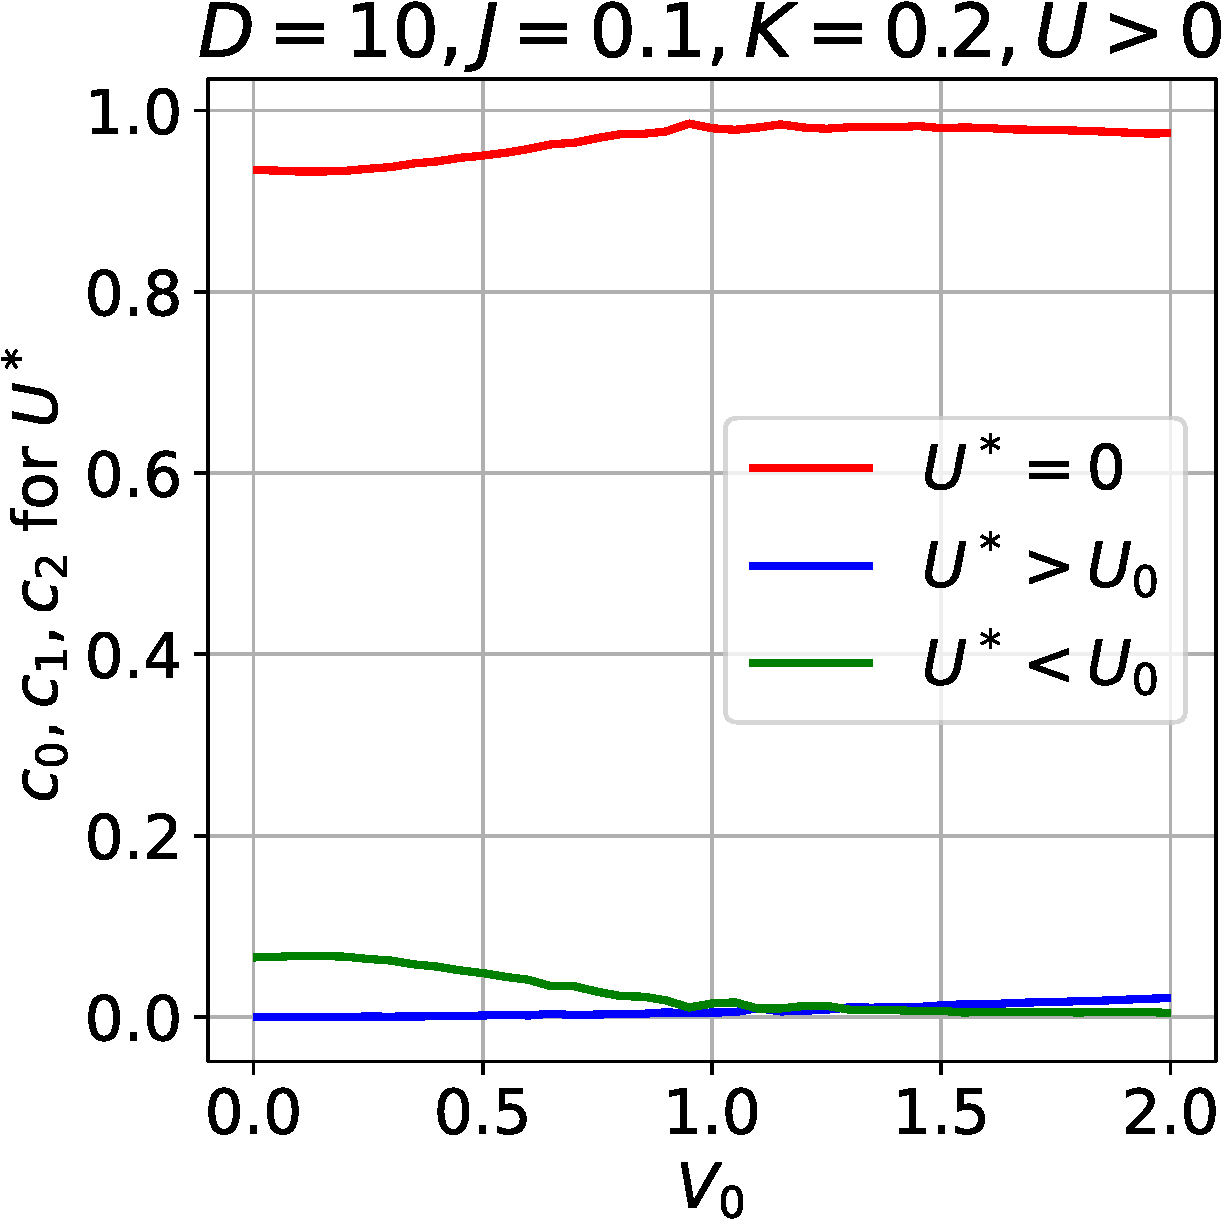
\includegraphics[scale=0.38]{../figures/quad2.pdf}
\end{minipage}
%\hspace{0.01\textwidth}
\begin{minipage}{.49\textwidth}
    \centering
    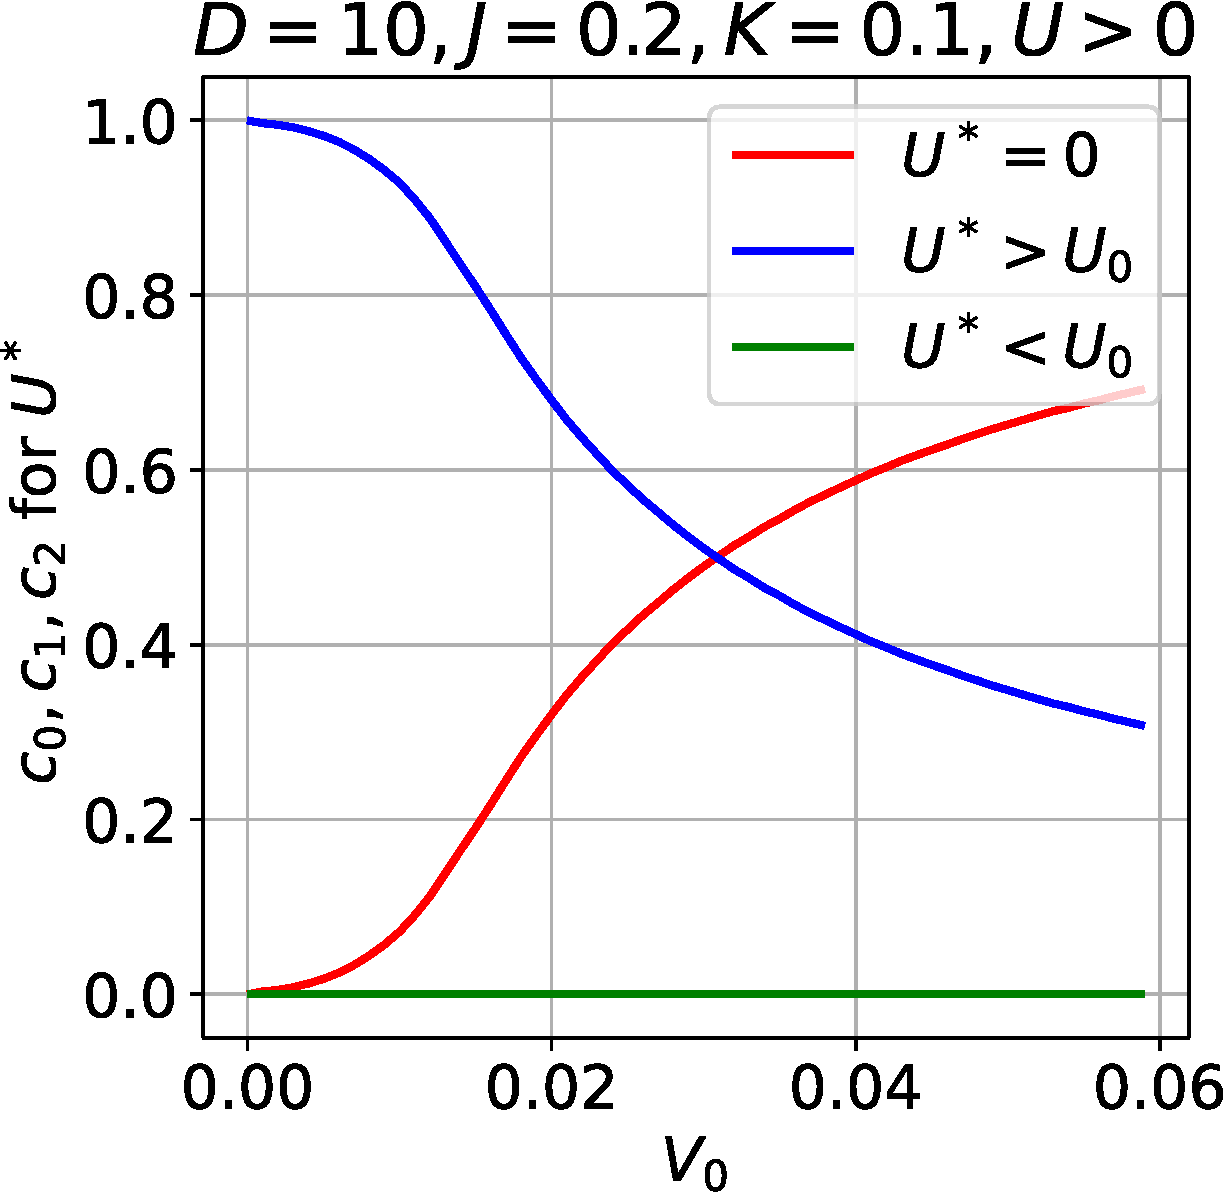
\includegraphics[scale=0.38]{../figures/quad1.pdf}
\end{minipage}

  \medskip

  \begin{minipage}{.49\textwidth}
    \centering
    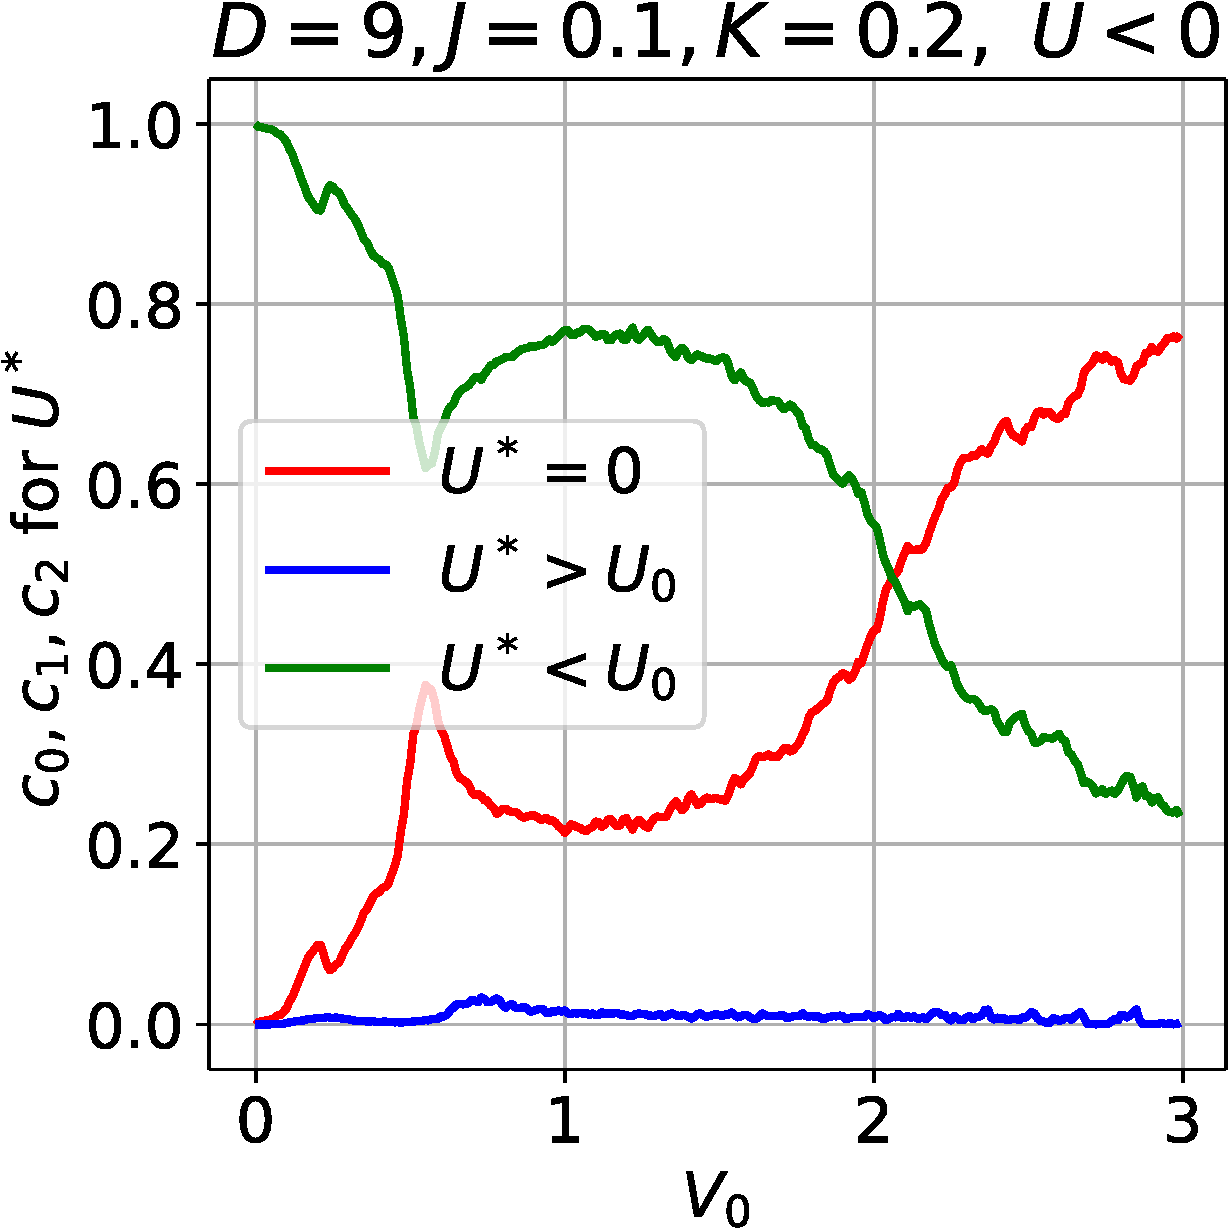
\includegraphics[scale=0.38]{../figures/quad3.pdf}
\end{minipage}
%\hspace{0.02\textwidth}
  \begin{minipage}{.49\textwidth}
    \centering
    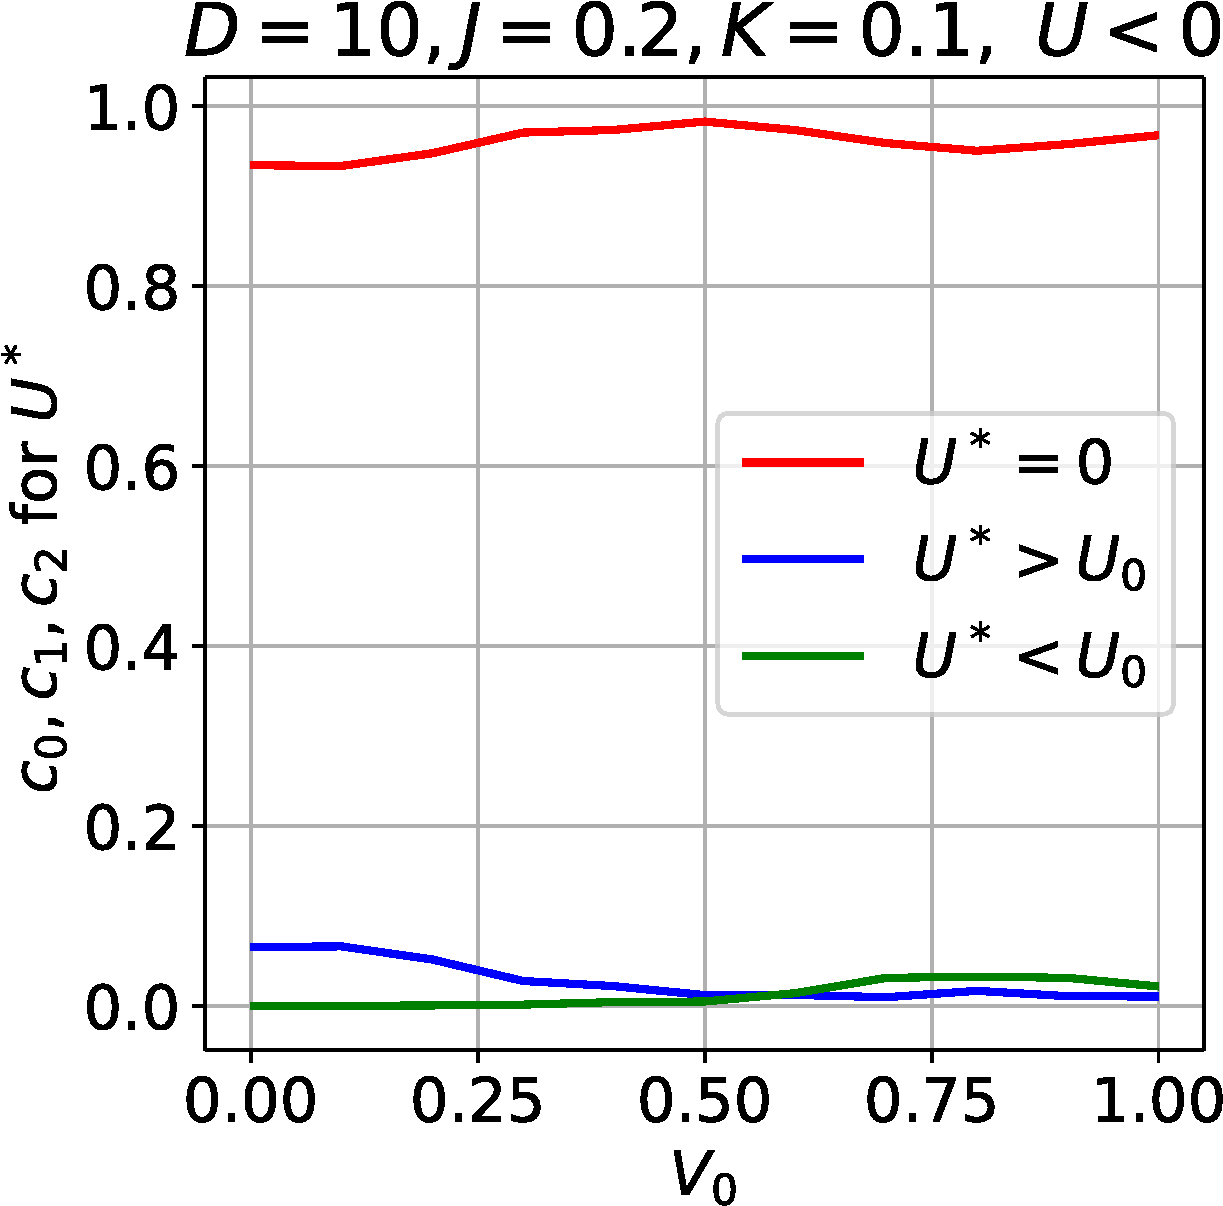
\includegraphics[scale=0.38]{../figures/quad4.pdf}
\end{minipage}
\label{Veffect}
\captionof{figure}{Fraction of fixed points with various values of \(U^*\), as a function of bare \(V\). Each quadrant represents the corresponding quadrant in the phase diagram fig.~\ref{siamphases}. First and third quadrants suffer a transition. Bare values are mentioned in plot titles. Calculations were performed for \(\omega \in \left[ - \frac{D_0}{2}, \frac{D_0}{2} \right] \) and \(U \in \left[ 0, 5 \right] \).}
\end{center}
}

\comm{
\subsection{Second and fourth quadrants}
The second and fourth quadrants - \( J<K, U>0 \) and \(J>K, U<0 \) respectively - are quite simple. They do not feauture any change in the fixed point nature of \(U\). \(U^*=0\)  remains the dominant nature, just as it was for \(V=0\). The fixed point value of \(V\) switches to \(V^*>V_0\) for an infinitesimal value, same as in the first quadrant. The competition between the relevant and irrelevant fixed point values of \(U^*\) and \(V^*\) is shown in figs.~\ref{q2_frac} and \ref{q4_frac}. The linear increase in the proportions of the \(U^*=0, V^*>V_0\) fixed points in the second quadrant, and of the \(U^* < U_0 < 0, V^*>V_0\) fixed points in the third quadrant signify that those are the ones that survive at large system size.
\pb We have also confirmed from our numerical studies that the fixed point value \(J^*\) for these two quadrants goes on increasing with the system size, suggesting that it flows to \(\infty\) in the thermodynamic limit, same as in the first quadrant. This is shown in fig.~\ref{J_D_q24}. The asymptotic behavior of \(V^*\) is, however, not so clear. These two quadrants are thus characterized by \(U^*=0\) and \(J,V\) relevant.
\begin{figure}[htpb!]
\centering
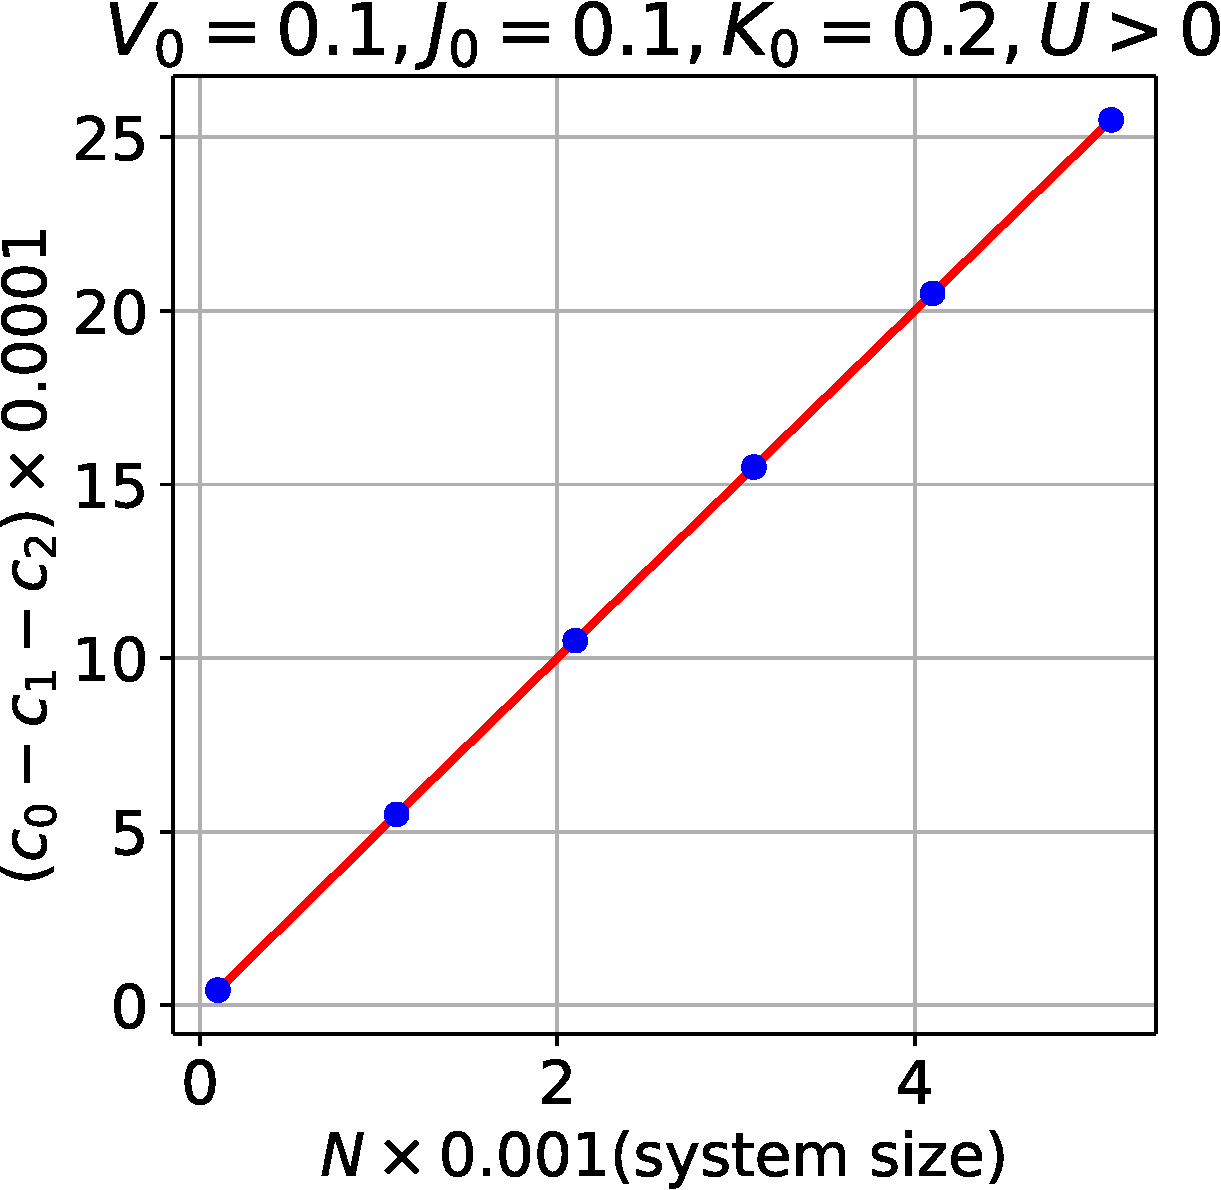
\includegraphics[scale=0.39]{../figures/frac_vs_D_quad2.pdf}
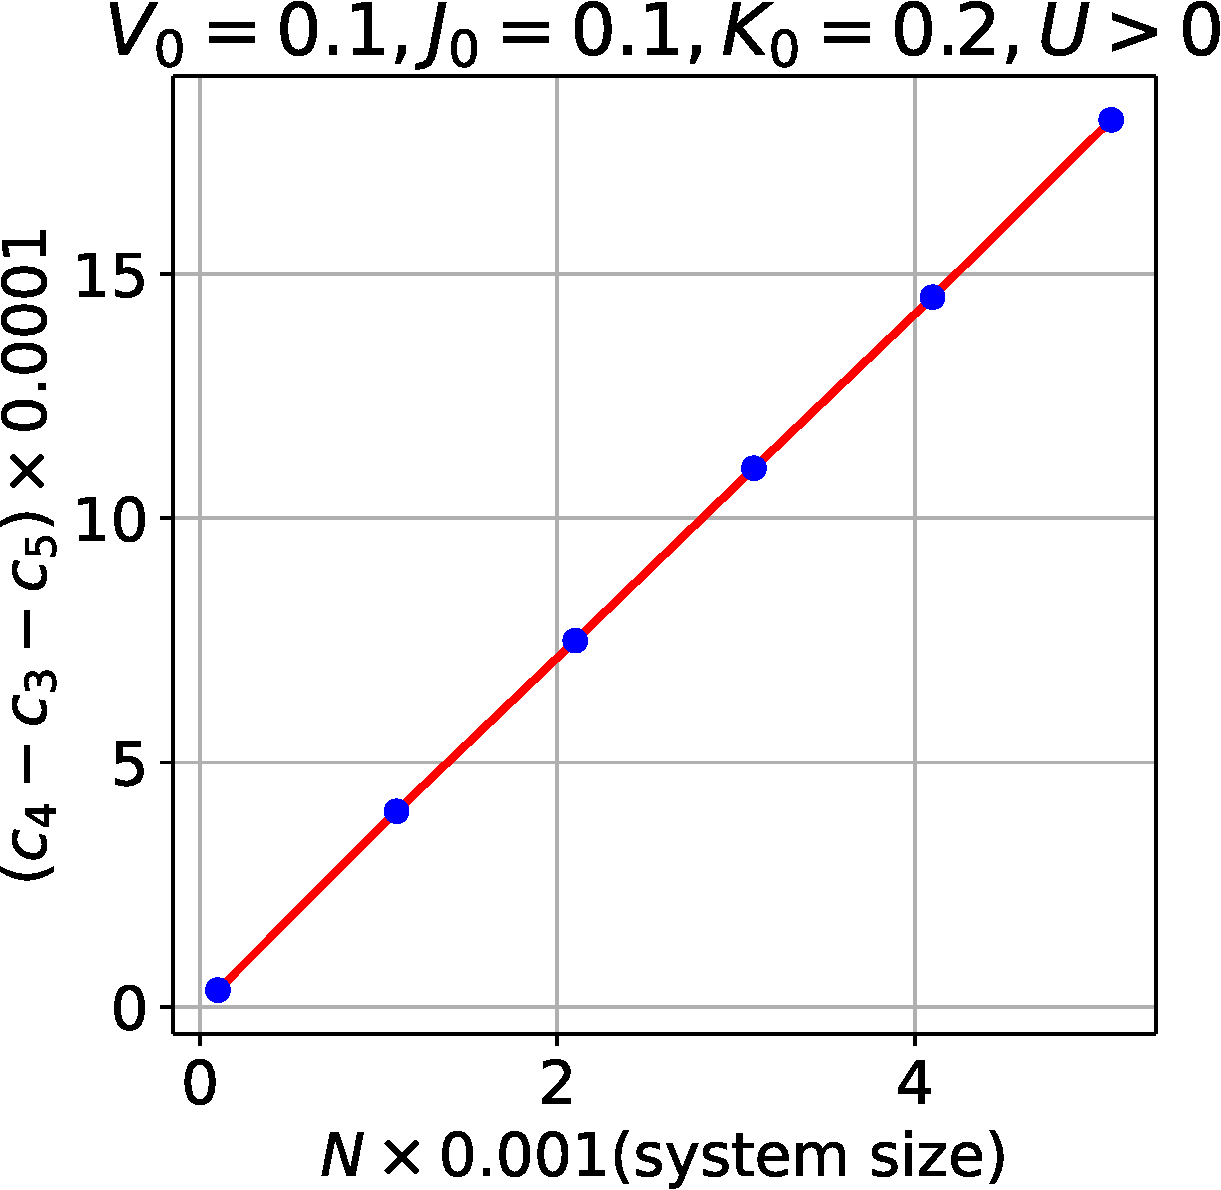
\includegraphics[scale=0.39]{../figures/frac_vs_D_quad22.pdf}
\caption{Difference in the number of fixed points for $U^*$ (left panel) and \(V^*\) (right panel), with the system size, for the second quadrant. All axes are in log scale.}
\label{q2_frac}
\end{figure}
\begin{figure}[htpb!]
\centering
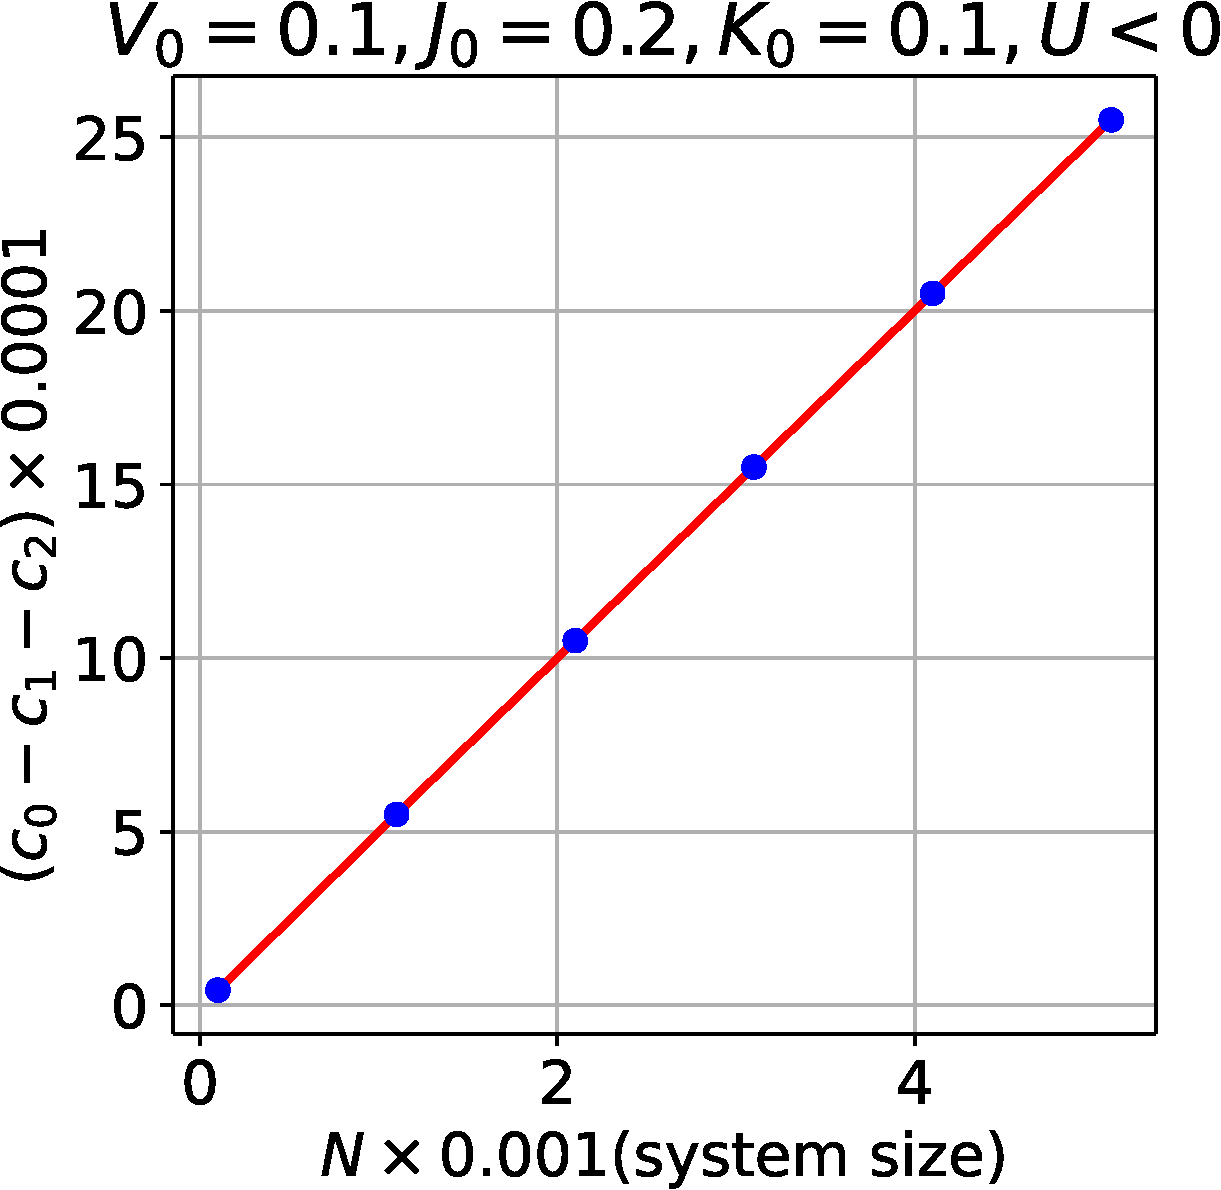
\includegraphics[scale=0.39]{../figures/frac_vs_D_quad4.pdf}
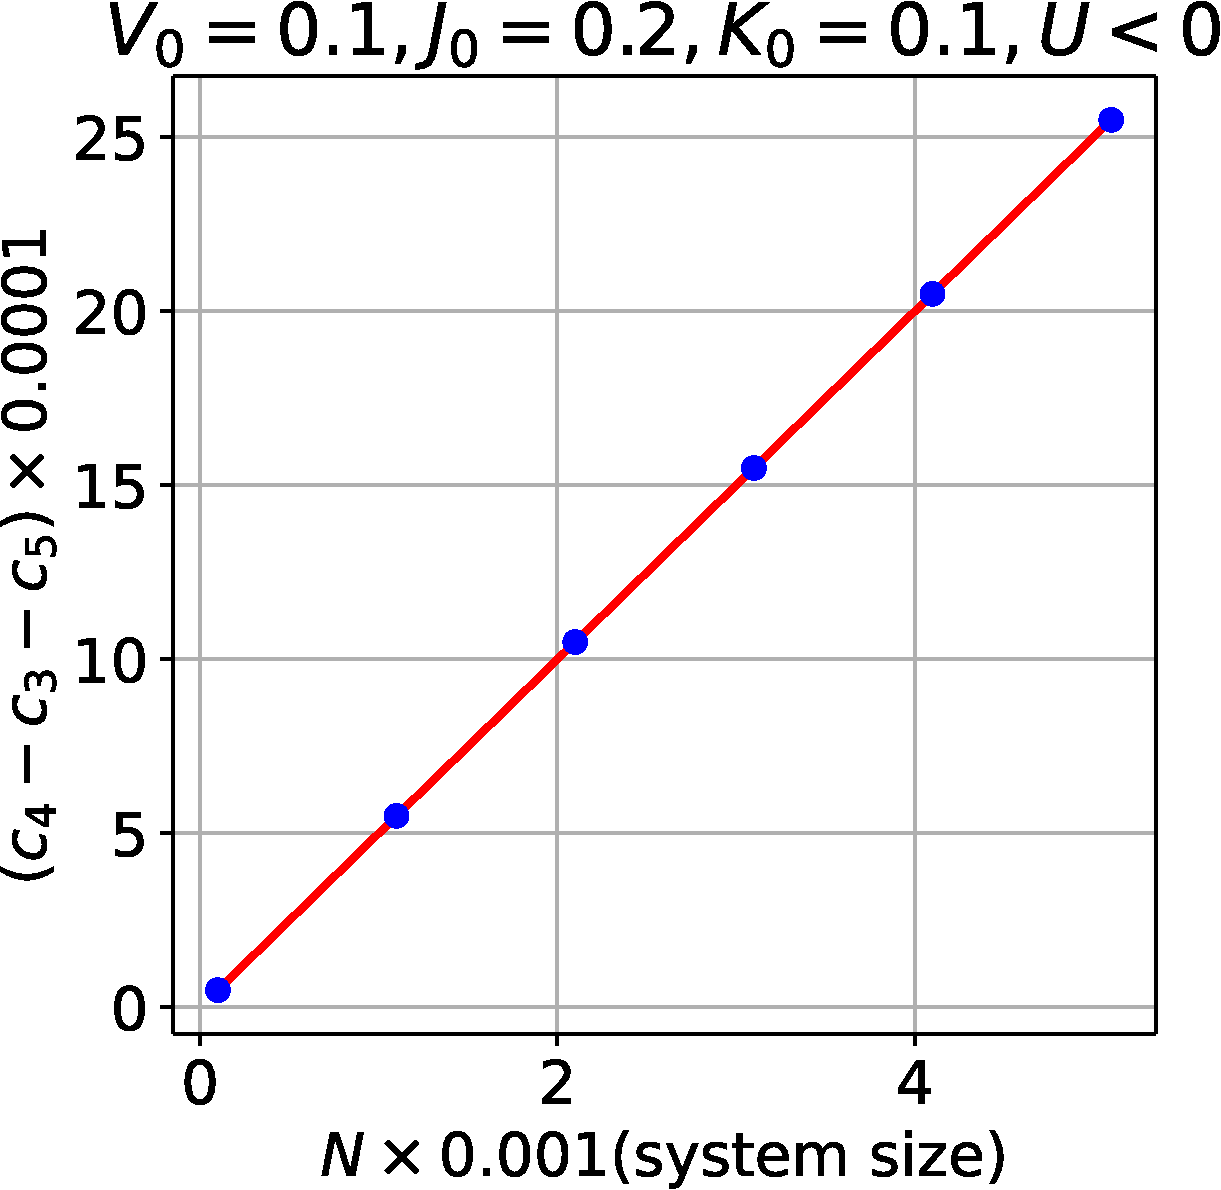
\includegraphics[scale=0.39]{../figures/frac_vs_D_quad44.pdf}
\caption{Difference in the number of fixed points for $U^*$ (left panel) and \(V^*\) (right panel), with the system size, for the fourth quadrant. All axes are in log scale.}
\label{q4_frac}
\end{figure}
\begin{figure}[htpb!]
\centering
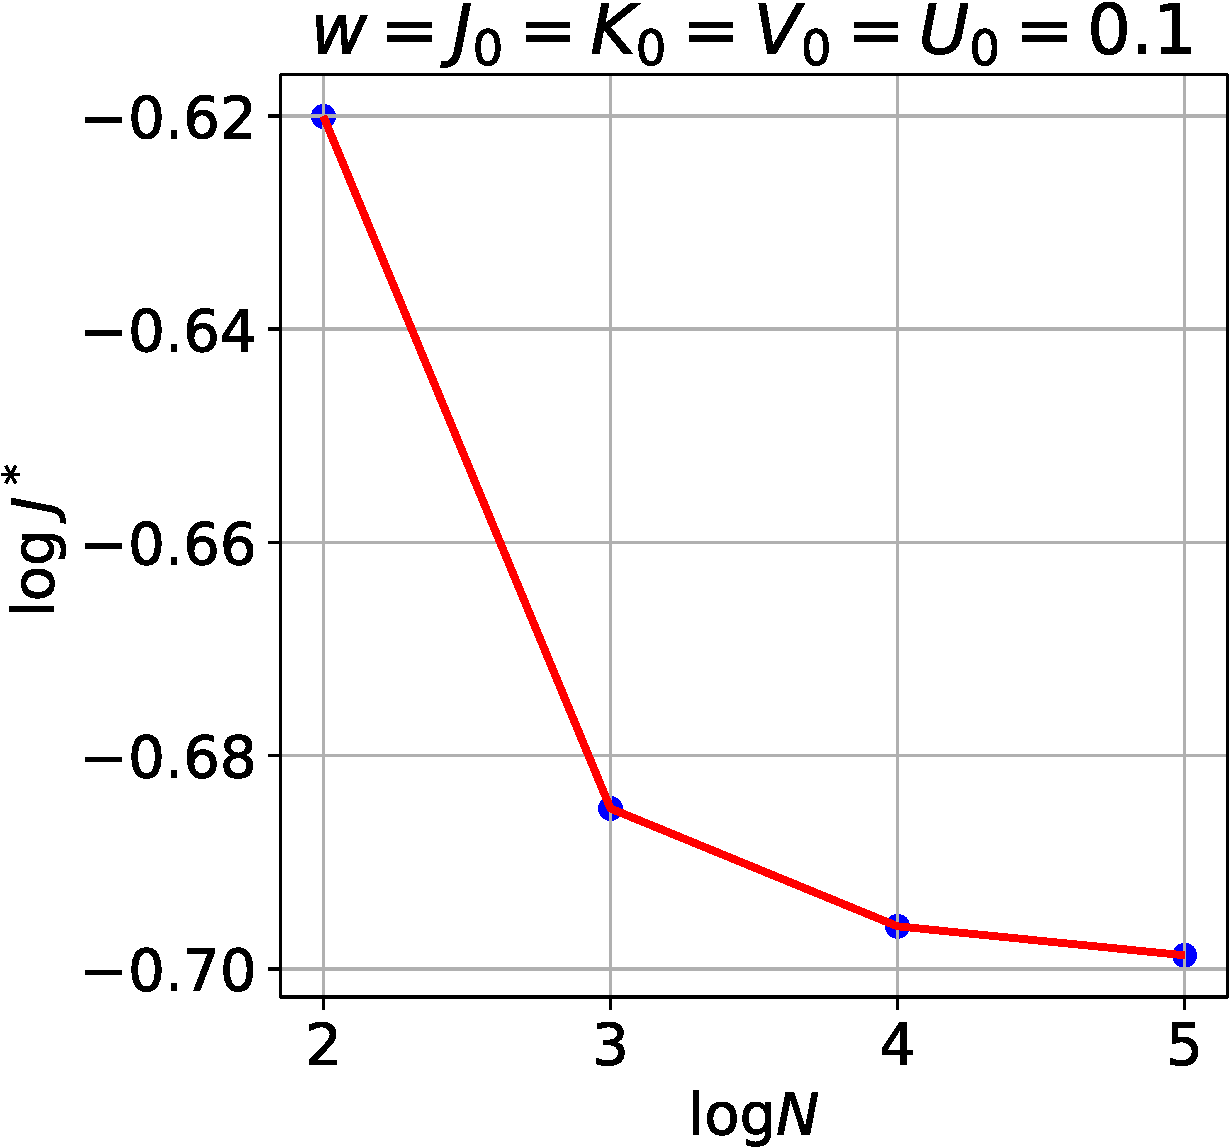
\includegraphics[scale=0.39]{../figures/J_vs_D_q2.pdf}
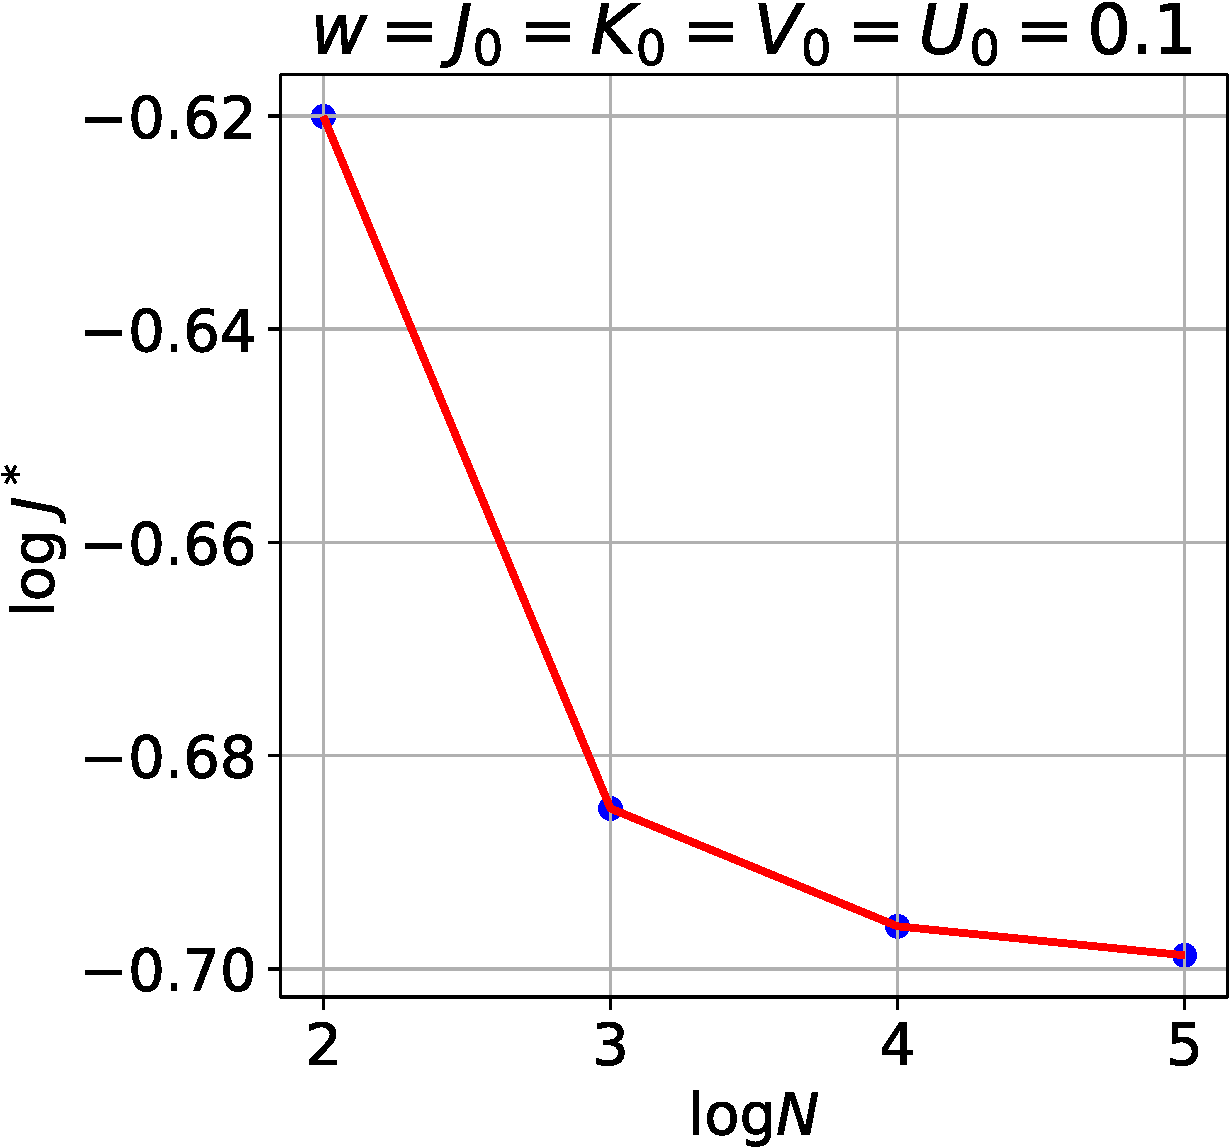
\includegraphics[scale=0.39]{../figures/J_vs_D_q4.pdf}
\caption{Variation of the fixed point value of $J^*$  with the system size, for the second (left panel) and fourth (right panel) quadrants. All axes are in log scale.}
\label{J_D_q24}
\end{figure}
}
